\setcounter{section}{2}
\section{GÓC Ở TÂM, GÓC NỘI TIẾP}
\subsection{Trọng tâm kiến thức}
\begin{tomtat}
\subsubsection{Góc ở tâm}
\begin{boxdn}
	\textit{Góc ở tâm} là góc có đỉnh trùng với tâm đường tròn.
\end{boxdn}
\subsubsection{Cung, số đo cung}
\paragraph{Cung}
\begin{boxdn}
Mỗi phần đường tròn giới hạn bởi hai điểm $A$, $B$ trên đường tròn gọi là một \textit{cung} $AB$, kí hiệu là $\wideparen{AB}$.
\begin{center}
	\begin{tikzpicture}[line join = round, line cap = round,>=stealth,scale=0.7]
	\clip (-2.1,-2.1) rectangle (2.1,2.5);
	\coordinate[label = below:$O$] (O) at (0,0);
	\coordinate[blue,label = above:$n$] (n) at (0,2);
	\coordinate[red,label = above:$m$] (m) at (0,-2);
	\coordinate[label = above:$A$] (A) at ($(0,0)+(120:2cm)$); 
	\coordinate[label = above:$B$] (B) at ($(0,0)+(60:2cm)$);
	\draw[blue] (B) arc (60:120:2 cm);
	\draw[red] (B) arc (60:-240:2 cm);	
	\draw (O)--(A) (O)--(B);
	\foreach \x in {O,A,B}
	\fill[black] (\x) circle (1.5pt);
	\end{tikzpicture}
	\hspace*{1cm}
	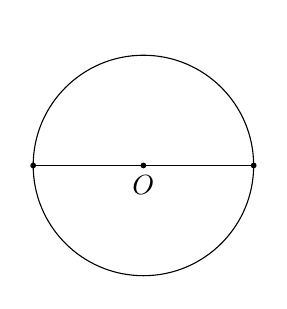
\begin{tikzpicture}[line join = round, line cap = round,>=stealth,scale=0.7]
	\clip (-2.1,-2.1) rectangle (2.1,2.5);
	\coordinate[label = below:$O$] (O) at (0,0);
	\coordinate[label = right:$E$] (E) at (0:2);
	\coordinate[label = left:$F$] (F) at (180:2);
	\draw (O) circle (2 cm);	
	\draw (E)--(F);
	\foreach \x in {O,E,F} \fill[black] (\x) circle (1.5pt);	
	\end{tikzpicture}
\end{center}
\begin{itemize}
	\item Trong hình trên, ta nói góc ở tâm $\widehat{AOB}$ chắn cung $AnB$ hay cung $AnB$ bị chắn bởi góc ở tâm $\widehat{AOB}$.\\
	Khi $0^{\circ}<\widehat{AOB}<180^{\circ}$, để phân biệt hai cung có chung các mút là $A$ và $B$, $\wideparen{AnB}$ là \textit{cung nhỏ} và $\wideparen{AmB}$ là \textit{cung lớn}.\\
	Khi $AB$ là đường kính thì gọi cung $AB$ là cung nửa đường tròn.
	\item Khi nói \lq\lq góc ở tâm $\widehat{AOB}$ chắn cung $AB$\rq\rq\ thì ta hiểu là góc ở tâm chắn cung nhỏ $AB$.
	\item Nếu $EF$ là đường kính thì mỗi cung $EF$ là một nửa đường tròn. Góc bẹt $\widehat{EOF}$ chắn nửa đường tròn.
\end{itemize}
\end{boxdn}
\paragraph{Số đo cung}
\begin{boxdn}
	\begin{itemize}
	\item Số đo của cung nhỏ bằng số đo của góc ở tâm chắn cung đó. Số đo của cung lớn bằng hiệu giữa $360^{\circ}$ và số đo của cung nhỏ có chung hai đầu mút với cung lớn.
	\item Số đo của cung nửa đường tròn bằng $180^{\circ}$.	
	\item Số đo của cung $AB$ được kí hiệu là sđ$\wideparen{AB}$.
	\end{itemize}
\end{boxdn}
\begin{note}
	\begin{enumerate}[\bf ---]
	\item Cung nhỏ có số đo nhỏ hơn $180^{\circ}$, cung lớn có số đo lớn hơn $180^{\circ}$. Cung nửa đường tròn có số đo $180^{\circ}$.
	\item Khi hai mút của cung trùng nhau, ta có \textit{cung không} với số đo $0^{\circ}$ và \textit{cung cả đường tròn} có số đo $360^{\circ}$.
	\item Một cung có số đo $n^{\circ}$ thường được gọi tắt là cung $n^{\circ}$.
	\item Trong một đường tròn, hai cung được gọi là bằng nhau nếu chúng có số đo bằng nhau.
	\end{enumerate}
\end{note}
\begin{boxdn}
	Trên đường tròn $(O)$, cho $B$ là một điểm nằm trên cung $AC$. Ta nói điểm $B$ chia cung $AC$ thành hai cung $\wideparen{AB}, \wideparen{BC}$. Một cách tổng quát, ta có
	\begin{center}
	sđ$\wideparen{AC}=\text{sđ}\wideparen{AB}+ \text{sđ} \wideparen{BC}$.
	\end{center}
\end{boxdn}
\subsubsection{Góc nội tiếp}
\paragraph{Nhận biết góc nội tiếp}
\begin{boxdn}
	\textit{Góc nội tiếp} là góc có đỉnh nằm trên đường tròn và hai cạnh chứa hai dây cung của đường tròn đó. Cung nằm bên trong góc được gọi là \textit{cung bị chắn}.
\end{boxdn}
\paragraph{Số đo góc nội tiếp}
\begin{boxdl}
	Trong một đường tròn, số đo của góc nội tiếp bằng nửa số đo của cung bị chắn.
\end{boxdl}
\begin{note}
	Trong một đường tròn
	\begin{enumerate}[\bf ---]
	\item Các góc nội tiếp bằng nhau chắn các cung bằng nhau.
	\item Các góc nội tiếp cùng chắn một cung hoặc chắn các cung bằng nhau thì bằng nhau.
	\item Góc nội tiếp nhỏ hơn hoặc bằng $90^{\circ}$ có số đo bằng nửa số đo của góc ở tâm cùng chắn một cung.
	\item Góc nội tiếp chắn nửa đường tròn là góc vuông.
	\end{enumerate}
\end{note}
\begin{center}
	\begin{tikzpicture}[line join = round, line cap = round,>=stealth,scale=0.8]
	\coordinate[label = left:$O$] (O) at (0,0);
	\coordinate[label = center:$a$] (a) at (0,-2.5);	\coordinate[label = right:$A$] (A) at (50:2);
	\coordinate[label = right:$B$] (B) at (-40:2);
	\coordinate[label = above:$M$] (M) at (110:2);
	\coordinate[label = left:$N$] (N) at (-2,0);
	\draw (O) circle (2 cm);	
	\draw (A)--(M) (A)--(N) (O)--(A) (O)--(B) (M)--(B) (N)--(B);
	\foreach \x in {O,A,B,M,N} \fill[black] (\x) circle (1.5pt);	
	\draw pic[draw,blue,angle radius=2mm,angle eccentricity=1.5] {angle = B--O--A};
	\draw pic[draw,blue,angle radius=2mm] {angle = B--M--A}
	pic[draw,blue,angle radius=4mm] {angle = B--M--A};
	\draw pic[draw,blue,angle radius=2mm] {angle = B--N--A}
	pic[draw,blue,angle radius=4mm] {angle = B--N--A};	 	
	\end{tikzpicture}
	\hspace*{1cm}
	\begin{tikzpicture}[line join = round, line cap = round,>=stealth,scale=0.8]
	\coordinate[label = below:$O$] (O) at (0,0);
	\coordinate[label = center:$b$] (b) at (0,-2.5);	\coordinate[label = right:$A$] (A) at (2,0);
	\coordinate[label = left:$B$] (B) at (-2,0);
	\coordinate[label = above:$M$] (M) at (130:2);
	\coordinate[label = above:$N$] (N) at (85:2);
	\coordinate[label = above:$P$] (P) at (50:2);
	\draw (O) circle (2 cm);	
	\draw (A)--(M) (A)--(N) (P)--(A) (M)--(B) (N)--(B) (P)--(B) (A)--(B);
	\foreach \x in {O,A,B,M,N,P} \fill[black] (\x) circle (1.5pt);	
	\draw pic[angle radius=2mm,draw=blue,fill=green!50,opacity=.3,angle eccentricity=1.5] {right angle = A--N--B}
	pic[angle radius=2mm,draw=blue,fill=green!50,opacity=.3,angle eccentricity=1.5] {right angle = A--M--B}
	pic[angle radius=2mm,draw=blue,fill=green!50,opacity=.3,angle eccentricity=1.5] {right angle = A--P--B}; 
	\end{tikzpicture}
\end{center}
\end{tomtat}
%%%%%%%%%%%%%%%%%%%
\subsection{Các dạng bài tập}
\begin{dang}{Nhận biết góc ở tâm, góc nội tiếp, cung tròn}
\end{dang}
\begin{vd}
	Trong các góc $AOB, CID, MON$ ở hình sau, góc nào là góc ở tâm, góc nào không là góc ở tâm?
	\begin{center}
	\begin{tikzpicture}[line join = round, line cap = round,>=stealth,font=\footnotesize,scale=0.6]
	\def\r{2}
	\path 
	(0,0) coordinate (O)
	(\r,0) coordinate (X)
	($(O)!1!-30:(X)$) coordinate (B)
	($(O)!1!30:(X)$) coordinate (A)
	;
	\draw (O) circle(\r cm);
	\draw (A)--(O)--(B);
	\foreach \x/\g in {O/180,A/30,B/-30}\fill[black] (\x) circle (1pt) ($(\x)+(\g:3mm)$) node{$\x$};
	\foreach \a/\b/\c in {B/O/A}{\draw pic[draw,angle radius=2mm] {angle = \a--\b--\c};}
	\path (current bounding box.south) node[below]{\bfseries a)};	
	\end{tikzpicture}\qquad
	%---------------------------------------------
	\begin{tikzpicture}[line join = round, line cap = round,>=stealth,font=\footnotesize,scale=0.6]
	\def\r{2}
	\path 
	(0,0) coordinate (O)
	(\r,0) coordinate (X)
	($(O)!1!30:(X)$) coordinate (C)
	($(O)!1!-60:(X)$) coordinate (I)
	($(O)!-1!(I)$) coordinate (D)
	;
	\draw (O) circle(\r cm);
	\draw (D)--(I)--(C);
	\foreach \x/\g in {O/-160,C/30,I/-60,D/120}\fill[black] (\x) circle (1pt) ($(\x)+(\g:3mm)$) node{$\x$};
	\foreach \a/\b/\c in {C/I/D}{\draw pic[draw,angle radius=2mm] {angle = \a--\b--\c};}
	\path (current bounding box.south) node[below=-1mm]{\bfseries b)};
	\end{tikzpicture}\qquad
	\begin{tikzpicture}[line join = round, line cap = round,>=stealth,font=\footnotesize,scale=0.6]
	\def\r{2}
	\path 
	(0,0) coordinate (O)
	(\r,0) coordinate (X)
	($(O)!1!180:(X)$) coordinate (M)
	($(O)!1!0:(X)$) coordinate (N)
	;
	\draw (O) circle(\r cm);
	\draw (M)--(N);
	\foreach \x/\g in {O/-90,M/180,N/0}\fill[black] (\x) circle (1pt) ($(\x)+(\g:3mm)$) node{$\x$};
	\foreach \a/\b/\c in {N/O/M}{\draw pic[draw,angle radius=2mm] {angle = \a--\b--\c};}
	\path (current bounding box.south) node[below]{\bfseries c)};	
	\end{tikzpicture}
	\end{center}
	\loigiai{
	Hai góc $AOB$ và $MON$ là góc ở tâm vì có đỉnh trùng với tâm đường tròn. Góc $CID$ không là góc ở tâm vì có đỉnh không trùng với tâm đường tròn.
	}
\end{vd}
\begin{vd}
	\immini{Trong hình bên, hãy cho biết:
	\begin{enumerate}
	\item Cung $AmB$ bị chắn bởi góc ở tâm nào?
	\item Góc ở tâm $AOC$ chắn cung nào?
	\end{enumerate}}
	{\begin{tikzpicture}[line join = round, line cap = round,>=stealth,font=\footnotesize,scale=0.6]
	\def\r{2}
	\path 
	(0,0) coordinate (O)
	(\r,0) coordinate (X)
	($(O)!1!80:(X)$) coordinate (A)
	($(O)!1!140:(X)$) coordinate (B)
	($(O)!1!170:(X)$) coordinate (C)
	;
	\draw (O) circle(\r cm);
	\draw (A)--(O)--(B) (O)--(C);
	\foreach \x/\g in {O/-30,A/80,B/110,C/160}\fill[black] (\x) circle (1pt) ($(\x)+(\g:3mm)$) node{$\x$};
	\draw (110:2) node[above]{m};
	\end{tikzpicture}}
	\loigiai{
	\begin{enumerate}
	\item Cung $AmB$ bị chắn bởi góc ở tâm $AOB$.
	\item Góc ở tâm $AOC$ chắn cung $ABC$.
	\end{enumerate}	}
\end{vd}
\begin{vd}
	\immini
	{Cho tam giác $MNP$ có ba đỉnh nằm trên đường tròn $(I)$. Xác định các góc ở tâm của đường tròn.
	}
	{\begin{tikzpicture}[line join = round, line cap = round,>=stealth,scale=0.7]
	\coordinate[label = left:$I$] (I) at (0,0);
	\coordinate[label = above:$M$] (M) at ($(0,0)+(120:2cm)$); 
	\coordinate[label = left:$N$] (N) at ($(0,0)+(-150:2cm)$);
	\coordinate[label = right:$P$] (P) at ($(0,0)+(-30:2cm)$);
	\draw (I) circle (2 cm);
	\draw (I)--(M) (I)--(N) (I)--(P) (M)--(N)--(P)--cycle;
	\foreach \x in {I,N,M,P}
	\fill[black] (\x) circle (1.5pt);	
	\end{tikzpicture}}
	\loigiai{Trong hình, đường tròn $(I)$ có các góc ở tâm là $\widehat{MIN}$, $\widehat{NIP}$, $\widehat{PIM}$.}
\end{vd}
\begin{vd}
	\immini{	
	Cho ba điểm $A$, $B$ và $C$ thuộc đường tròn $(O)$ như hình bên.
	\begin{enumerate}
	\item Tìm các góc ở tâm có hai cạnh đi qua hai trong ba điểm $A$, $B$, $C$.
	\item Tìm các cung có hai mút là hai trong ba điểm $A$, $B$, $C$.
	\end{enumerate}}
	{
	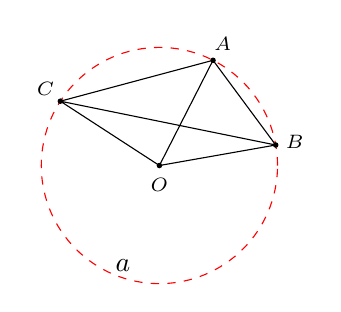
\begin{tikzpicture}[declare function={r=1.5;ga=63;gb=10;gc=147;}]
	\path (0,0) coordinate (O) %tam
	(ga:r) coordinate (A)
	(gb:r) coordinate (B)
	(gc:r) coordinate (C)
	(-110:0.9*r) coordinate (T)	;
	\draw[dashed,red] (O) circle (r);
	\draw (A)--(B)--(O)--(C)--cycle--(O) (B)--(C);
	\foreach \t/\g in {A/60,B/10,C/140,O/-90}{
	\fill (\t) circle (1pt) node[shift={(\g:7pt)},font=\scriptsize]{$ \t $};	}
	\node at (T) {$a$};
	\end{tikzpicture}}
	\loigiai{
	\begin{enumerate}
	\item Các góc ở tâm cần tìm là $\widehat{AOB}$, $\widehat{BOC}$ và $\widehat{COA}$.
	\item Các cung có hai mút $A$, $B$ là $\wideparen{AB}$, $\wideparen{ACB}$.
	\begin{itemize}
	\item Các cung có hai mút $A$, $C$ là $\wideparen{AC}$, $\wideparen{ABC}$.
	\item Các cung có hai mút $B$, $C$ là $\wideparen{BAC}$, $\wideparen{BaC}$.
	\end{itemize}
	\end{enumerate}}	
\end{vd}
\begin{vd}
	Quan sát các hình $a$, $b$, $c$, $d$, góc ở hình nào là góc nội tiếp, góc ở hình nào không là góc nội tiếp? Vì sao?
	\begin{center}
	\begin{tikzpicture}[line join = round, line cap = round,>=stealth,font=\footnotesize,scale=0.7]
	\def\r{1.5}
	\path 
	(0,0) coordinate (O)
	(\r,0) coordinate (X)
	($(O)!1!-150:(X)$) coordinate (A)
	($(O)!1!-30:(X)$) coordinate (B)
	($(O)!1!110:(X)$) coordinate (I)
	;
	\draw (O) circle(\r cm);
	\draw (A)--(I)--(B);
	\draw[fill] (O) circle(1.5pt);
	\foreach \a/\b/\c in {A/I/B}{\draw pic[draw,angle radius=2mm] {angle = \a--\b--\c};}
	\path (current bounding box.south) node[below]{a)};	
	\end{tikzpicture}\qquad
	\begin{tikzpicture}[line join = round, line cap = round,>=stealth,font=\footnotesize,scale=0.7]
	\def\r{1.5}
	\path 
	(0,0) coordinate (O)
	(\r,0) coordinate (X)
	($(O)!1!-150:(X)$) coordinate (A)
	($(O)!1!-30:(X)$) coordinate (B)
	($(O)!0.6!135:(X)$) coordinate (I)
	;
	\draw (O) circle(\r cm);
	\draw (A)--(I)--(B);
	\draw[fill] (O) circle(1.5pt);
	\foreach \a/\b/\c in {A/I/B}{\draw pic[draw,angle radius=2mm] {angle = \a--\b--\c};}
	\path (current bounding box.south) node[below]{b)};	
	\end{tikzpicture}\qquad
	\begin{tikzpicture}[line join = round, line cap = round,>=stealth,font=\footnotesize,scale=0.7]
	\def\r{1.5}
	\path 
	(0,0) coordinate (O)
	(\r,0) coordinate (X)
	($(O)!1!-150:(X)$) coordinate (A)
	($(O)!2!60:(X)$) coordinate (B)
	($(O)!1!110:(X)$) coordinate (I)
	;
	\draw (O) circle(\r cm);
	\draw (A)--(I)--(B);
	\draw[fill] (O) circle(1.5pt);
	\foreach \a/\b/\c in {A/I/B}{\draw pic[draw,angle radius=2mm] {angle = \a--\b--\c};}
	\path (current bounding box.south) node[below]{c)};	
	\end{tikzpicture}\qquad
	\begin{tikzpicture}[line join = round, line cap = round,>=stealth,font=\footnotesize,scale=0.7]
	\def\r{1.5}
	\path 
	(0,0) coordinate (O)
	(\r,0) coordinate (X)
	($(O)!2!10:(X)$) coordinate (A)
	($(O)!2!60:(X)$) coordinate (B)
	($(O)!1!50:(X)$) coordinate (I)
	;
	\draw (O) circle(\r cm);
	\draw (A)--(I)--(B);
	\draw[fill] (O) circle(1.5pt);
	\foreach \a/\b/\c in {A/I/B}{\draw pic[draw,angle radius=2mm] {angle = \a--\b--\c};}
	\path (current bounding box.south) node[below]{d)};	
	\end{tikzpicture}
	\end{center}
	\loigiai{
	Góc ở Hình $56a$ là góc nội tiếp vì góc có đỉnh thuộc đường tròn và hai cạnh chứa hai dây cung của đường tròn đó.\\
	Góc ở Hình $56b$ không là góc nội tiếp vì đỉnh không thuộc đường tròn.\\
	Góc ở Hình $56c$ không là góc nội tiếp vì một cạnh không chứa dây cung.\\
	Góc ở Hình $56d$ không là góc nội tiếp vì cả hai cạnh không chứa dây cung.
	}
\end{vd}
\begin{vd}
	Cho hai điểm $E$ và $F$ nằm trên đường tròn $(O)$. Có bao nhiêu góc nội tiếp chắn cung $EF$?
	\loigiai{Với mỗi điểm $M$ bất kì thuộc đường tròn ta xác định được góc $\widehat{EMF}$ là góc nội tiếp đường tròn $(O)$ chắn cung $EF$. Có vô số điểm $M$ như vậy nên có vô số góc nội tiếp chắn cung $EF$.}
\end{vd}
\begin{vd}
	\immini{Tìm góc nội tiếp chắn cung $AB$ của đường tròn $(O)$ trong Hình $9$.}
	{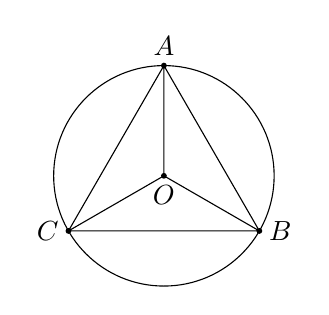
\begin{tikzpicture}[line join = round, line cap = round,>=stealth,scale=0.7]
	\coordinate[label = below:$O$] (O) at (0,0);
	\coordinate[label = above:$A$] (A) at (0,2);
	\coordinate[label = right:$B$] (B) at (-30:2);
	\coordinate[label = left:$C$] (C) at (-150:2);
	\draw (O) circle (2 cm);	
	\draw (O)--(B) (O)--(A) (O)--(C) (A)--(B)--(C)--cycle;
	\foreach \x in {O,A,B,C} \fill[black] (\x) circle (1.5pt);	
	\end{tikzpicture}}
	\loigiai{
	Trong hình, $\widehat{ACB}$ là góc nội tiếp chắn $\wideparen{AB}$ của đường tròn $(O)$.
	}
\end{vd}
\begin{vd}
	Cho tam giác đều $MNP$ có ba đỉnh nằm trên đường tròn $(I)$. Hãy chỉ ra các góc nội tiếp của đường tròn $(I)$ và tính số đo của các góc nội tiếp đó.
	\loigiai{
	\immini{
	Theo Hình $10$, ta có $\widehat{MNP}$, $\widehat{NPM}$ và $\widehat{NMP}$ là các góc nội tiếp của đường tròn $(I)$.\\
	Vì $MNP$ là tam giác đều nên $\widehat{MNP}=\widehat{NPM}=\widehat{NMP}=60^{\circ}$.
	}
	{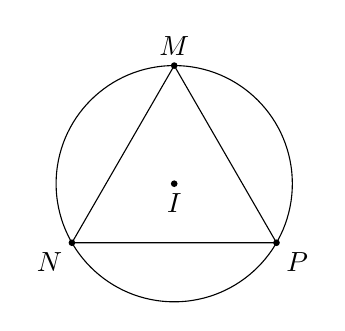
\begin{tikzpicture}[line join = round, line cap = round, scale=1] 
	\def \R{1.5}; 
	\coordinate[label = below left:$N$] (N) at (-150:\R); 
	\coordinate[label = below right:$P$] (P) at (-30:\R); 
	\coordinate[label = above:$M$] (M) at (90:\R);
	\coordinate[label = below:$I$] (I) at (0,0);
	\draw (I) circle (\R cm);
	\draw (M)--(N)--(P)--cycle;
	\foreach \x in {M,N,P,I} \fill[black] (\x) circle (1.2pt); 
	\end{tikzpicture} }
	}
\end{vd}
%====================
\begin{dang}{Tính số đo góc ở tâm, số đo cung tròn}
\end{dang}
\begin{vd}
	Tính số đo góc ở tâm được tạo thành khi kim giờ quay
	\begin{listEX}[2]
	\item Từ $7$ giờ đến $9$ giờ;
	\item Từ $9$ giờ đến $12$ giờ.
	\end{listEX}
	\loigiai{
	Cứ mỗi giờ, kim giờ quay được một góc là $360^{\circ} : 12=30^{\circ}$.
	\begin{listEX}[1]
	\item Từ $7$ giờ đến $9$ giờ, kim giờ quay được một góc $30^{\circ}\cdot 2=60^{\circ}$.
	\item Từ $9$ giờ đến $12$ giờ, kim giờ quay được một góc $30^{\circ}\cdot 3=90^{\circ}$.
	\end{listEX}
	}
\end{vd}
\begin{vd}
	Trong hình sau, coi mỗi khung đồng hồ là một đường tròn, kim giờ, kim phút là các tia. Số đo góc ở tâm trong mỗi hình $a, b, c, d$ là bao nhiêu?
	\begin{center}
	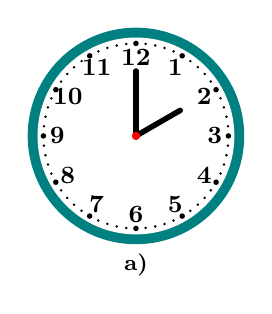
\begin{tikzpicture}[line join = round, line cap = round,>=stealth,font=\footnotesize,scale=0.25]
	\fill[teal] (0,0) circle (5.5);\fill[white!80] (0,0) circle (5);
	\foreach \angle/\nhan in {0/3, 30/2, 60/1, 90/12, 120/11, 150/10, 180/9, 210/8, 240/7, 270/6, 300/5, 330/4}{
	\draw (\angle:4) node{\small{\textbf{\color{black}\nhan}}};
	\fill[black] (\angle:4.7) circle (4pt);
	}
	\draw[line width=2pt,black] (-150:0)--(30:2.6);%Kim giờ
	\draw[line width=2pt,black] (-90:0)--(90:3.3);%Kim phút
	%\draw[line width=1pt,red] (90:1)--(270:3.6);
	\fill[red] (0,0) circle (6pt);
	\foreach \angle in {6,12,...,24}
	\foreach \rotate in {0,30,...,330}\fill[black] (\angle+\rotate:4.7) circle (2pt);
	\path (current bounding box.south) node[below]{\bfseries a)};
	\end{tikzpicture}\qquad
	%------------------------------------------------
	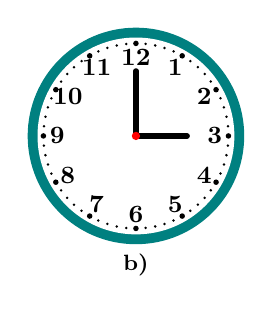
\begin{tikzpicture}[line join = round, line cap = round,>=stealth,font=\footnotesize,scale=0.25]
	\fill[teal] (0,0) circle (5.5);\fill[white!80] (0,0) circle (5);\foreach \angle/\label in {0/3, 30/2, 60/1, 90/12, 120/11, 150/10, 180/9, 210/8, 240/7, 270/6, 300/5, 330/4}{\draw (\angle:4) node{\small{\textbf{\color{black}\label}}};\fill[black] (\angle:4.7) circle (4pt);}
	\draw[line width=2pt,black] (-150:0)--(0:2.6);%Kim giờ
	\draw[line width=2pt,black] (-90:0)--(90:3.3);%Kim phút
	%\draw[line width=1pt,red] (90:1)--(270:3.6);
	\fill[red] (0,0) circle (6pt);
	\foreach \angle in {6,12,...,24}
	\foreach \rotate in {0,30,...,330}\fill[black] (\angle+\rotate:4.7) circle (2pt);
	\path (current bounding box.south) node[below]{\bfseries b)};
	\end{tikzpicture}\qquad
	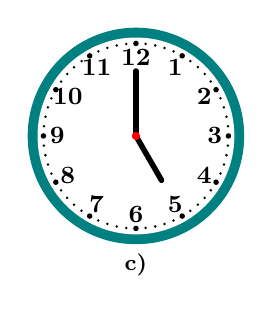
\begin{tikzpicture}[line join = round, line cap = round,>=stealth,font=\footnotesize,scale=0.25]
	\fill[teal] (0,0) circle (5.5);\fill[white!80] (0,0) circle (5);\foreach \angle/\label in {0/3, 30/2, 60/1, 90/12, 120/11, 150/10, 180/9, 210/8, 240/7, 270/6, 300/5, 330/4}{\draw (\angle:4) node{\small{\textbf{\color{black}\label}}};\fill[black] (\angle:4.7) circle (4pt);}
	\draw[line width=2pt,black] (-150:0)--(-60:2.6);%Kim giờ
	\draw[line width=2pt,black] (-90:0)--(90:3.3);%Kim phút
	%\draw[line width=1pt,red] (90:1)--(270:3.6);
	\fill[red] (0,0) circle (6pt);
	\foreach \angle in {6,12,...,24}
	\foreach \rotate in {0,30,...,330}\fill[black] (\angle+\rotate:4.7) circle (2pt);
	\path (current bounding box.south) node[below]{\bfseries c)};
	\end{tikzpicture}\qquad
	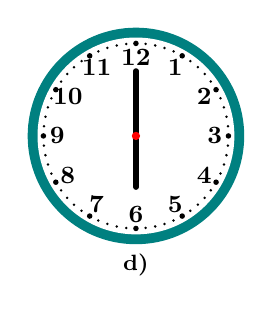
\begin{tikzpicture}[line join = round, line cap = round,>=stealth,font=\footnotesize,scale=0.25]
	\fill[teal] (0,0) circle (5.5);\fill[white!80] (0,0) circle (5);\foreach \angle/\label in {0/3, 30/2, 60/1, 90/12, 120/11, 150/10, 180/9, 210/8, 240/7, 270/6, 300/5, 330/4}{\draw (\angle:4) node{\small{\textbf{\color{black}\label}}};\fill[black] (\angle:4.7) circle (4pt);}
	\draw[line width=2pt,black] (-150:0)--(-90:2.6);%Kim giờ
	\draw[line width=2pt,black] (-90:0)--(90:3.3);%Kim phút
	%\draw[line width=1pt,red] (90:1)--(270:3.6);
	\fill[red] (0,0) circle (6pt);
	\foreach \angle in {6,12,...,24}
	\foreach \rotate in {0,30,...,330}\fill[black] (\angle+\rotate:4.7) circle (2pt);
	\path (current bounding box.south) node[below]{\bfseries d)};
	\end{tikzpicture}
	\end{center}
	\loigiai{
	\begin{enumerate}
	\item Hình a): Góc ở tâm tạo bởi kim giờ và kim phút tạo thành góc có số đo bằng $60^{\circ}$.
	\item Hình b): Góc ở tâm tạo bởi kim giờ và kim phút tạo thành góc có số đo bằng $90^{\circ}$.
	\item Hình c): Góc ở tâm tạo bởi kim giờ và kim phút tạo thành góc có số đo bằng $150^{\circ}$.
	\item Hình d): Góc ở tâm tạo bởi kim giờ và kim phút tạo thành góc có số đo bằng $180^{\circ}$.
	\end{enumerate}
	}
\end{vd}
\begin{vd}
	\immini{
	Tính số đo các cung $\wideparen{AnB}$ và $\wideparen{AmB}$ trong hình bên.
	}{
	\begin{tikzpicture}[line join = round, line cap = round,>=stealth,scale=0.7]
	\coordinate[label = below:$O$] (O) at (0,0);
	\coordinate[label = right:$A$] (A) at (2,0);
	\coordinate[label = above:$B$] (B) at (60:2);
	\coordinate[label = center:$n$] (n) at (1.9,1.3);
	\coordinate[label = center:$m$] (m) at (-1.8,-1.5);
	\draw (O) circle (2 cm);	
	\draw (O)--(B) (O)--(A);
	\foreach \x in {O,A,B} \fill[black] (\x) circle (1.5pt);	
	\draw pic[draw,blue,angle radius=4mm,angle eccentricity=2,"{\small $60^\circ$}"] {angle = A--O--B};	
	\end{tikzpicture}
	}
	\loigiai{
	Trong hình, ta có $\wideparen{AnB}$ bị chắn bởi góc ở tâm $\widehat{AOB}$ có số đo bằng $60^{\circ}$, suy ra sđ$\wideparen{AnB}=60^{\circ}$ và sđ$\wideparen{AmB}=360^{\circ}-60^{\circ}=300^{\circ}$.
	}
\end{vd}
\begin{vd}
	Trong hình sau, coi mỗi vành đồng hồ là một đường tròn. Tìm số đo của cung nhỏ $AB$ và cung lớn $CD$.
	\begin{center}
	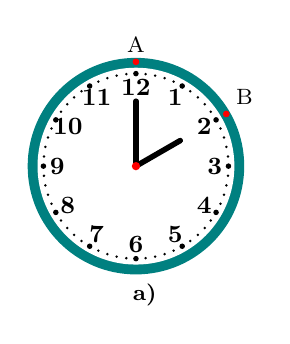
\begin{tikzpicture}[line join = round, line cap = round,>=stealth,font=\footnotesize,scale=0.25]
	\fill[teal] (0,0) circle (5.5);\fill[white!80] (0,0) circle (5);\foreach \angle/\label in {0/3, 30/2, 60/1, 90/12, 120/11, 150/10, 180/9, 210/8, 240/7, 270/6, 300/5, 330/4}{\draw (\angle:4) node{\small{\textbf{\color{black}\label}}};\fill[black] (\angle:4.7) circle (4pt);}
	\draw[line width=2pt,black] (-150:0)--(30:2.6);%Kim giờ
	\draw[line width=2pt,black] (-90:0)--(90:3.3);%Kim phút
	%\draw[line width=1pt,red] (90:1)--(270:3.6);
	\fill[red] (0,0) circle (6pt);
	\foreach \angle in {6,12,...,24}
	\foreach \rotate in {0,30,...,330}\fill[black] (\angle+\rotate:4.7) circle (2pt);
	\draw[fill,red] (90:5.3) circle(4pt) node[above, black]{A};
	\draw[fill,red] (30:5.3) circle(4pt) node[above right, black]{B};
	\path (current bounding box.south) node[below]{\bfseries a)};
	\end{tikzpicture}\qquad
	%------------------------------------------------
	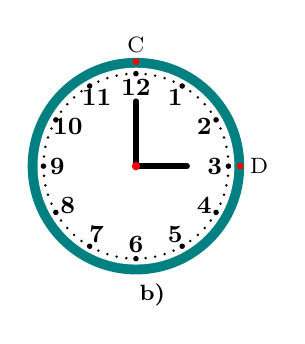
\begin{tikzpicture}[line join = round, line cap = round,>=stealth,font=\footnotesize,scale=0.25]
	\fill[teal] (0,0) circle (5.5);\fill[white!80] (0,0) circle (5);\foreach \angle/\label in {0/3, 30/2, 60/1, 90/12, 120/11, 150/10, 180/9, 210/8, 240/7, 270/6, 300/5, 330/4}{\draw (\angle:4) node{\small{\textbf{\color{black}\label}}};\fill[black] (\angle:4.7) circle (4pt);}
	\draw[line width=2pt,black] (-150:0)--(0:2.6);%Kim giờ
	\draw[line width=2pt,black] (-90:0)--(90:3.3);%Kim phút
	%\draw[line width=1pt,red] (90:1)--(270:3.6);
	\fill[red] (0,0) circle (6pt);
	\foreach \angle in {6,12,...,24}
	\foreach \rotate in {0,30,...,330}\fill[black] (\angle+\rotate:4.7) circle (2pt);
	\draw[fill,red] (90:5.3) circle(4pt) node[above, black]{C};
	\draw[fill,red] (0:5.3) circle(4pt) node[right, black]{D};
	\path (current bounding box.south) node[below]{\bfseries b)};
	\end{tikzpicture}
	\end{center}
	\loigiai{
	\begin{itemize}
	\item Vì số đo của cung cả đường tròn gấp sáu lần số đo cung nhỏ $AB$ và cung cả đường tròn có số đo $360^{\circ}$ nên
	$$
	\text{sđ } \wideparen{AB}=\dfrac{1}{6}\cdot 360^{\circ}=60^{\circ}.
	$$
	\item Vì số đo của cung cả đường tròn gấp bốn lần số đo cung nhỏ $CD$ và cung cả đường tròn có số đo $360^{\circ}$ nên
	$$
	\text{sđ } \wideparen{CD}=\dfrac{1}{4}\cdot 360^{\circ}=90^{\circ}.
	$$
	\end{itemize}
	Vậy $\text{sđ }\wideparen{CnD}=360^{\circ}-90^{\circ}=270^{\circ}$.
	}
\end{vd}
\begin{vd}
	Trên cung $AB$ có số đo $90^{\circ}$ của đường tròn $(O)$, lấy điểm $M$ sao cho cung $AM$ có số đo $15^{\circ}$. Tính số đo của cung $MB$.
	\loigiai{
	Vì sđ$\wideparen{AM}<$ sđ$\wideparen{MB}$ nên điểm $M$ nằm giữa $A$ và $B$.\\
	Do đó ta có $\text{sđ}\wideparen{AB}=\text{sđ}\wideparen{AM}+ \text{sđ} \wideparen{MB}$.\\
	Suy ra $\text{sđ} \wideparen{MB}=\text{sđ}\wideparen{AB}-\text{sđ}\wideparen{AM}=90^{\circ}-15^{\circ}=75^{\circ}$.
	}
\end{vd}
\begin{vd}
	\immini
	{Cho đường tròn $(O)$ có hai đường kính $AB$ và $CD$ vuông góc với nhau. Xác định số đo của các cung $\wideparen{AB}$, $\wideparen{AC}$ và $\wideparen{AD}$.}
	{\begin{tikzpicture}[line join = round, line cap = round,>=stealth,scale=0.7]
	\coordinate[label = below left:$O$] (O) at (0,0);
	\coordinate[label = right:$A$] (A) at (2,0);
	\coordinate[label = left:$B$] (B) at (-2,0);
	\coordinate[label = above:$C$] (C) at (0,2);
	\coordinate[label = below:$D$] (D) at (0,-2);
	\draw (O) circle (2 cm);	
	\draw (A)--(B) (C)--(D);
	\foreach \x in {O,A,B,C,D} \fill[black] (\x) circle (1.5pt);	
	\draw pic[angle radius=2mm] {right angle = A--O--C}; 
	\end{tikzpicture}}
	\loigiai{
	\begin{itemize}
	\item Vì $AB$ là đường kính của đường tròn $(O)$ nên cung $\wideparen{AB}$ là cung nửa đường tròn. \\
	Do đó sđ$\wideparen{AB}=180^{\circ}$.
	\item Ta có $\widehat{AOC}=90^{\circ}$ là góc ở tâm chắn cung $\wideparen{AC}$.\\
	Suy ra cung nhỏ $\wideparen{AC}$ có sđ$\wideparen{AC}=90^{\circ}$ và cung lớn $\wideparen{AC}$ có sđ$\wideparen{ADC}=360^{\circ}-90^{\circ}=270^{\circ}$.
	\item Ta có $\widehat{AOD}=90^{\circ}$ là góc ở tâm chắn cung $\wideparen{AD}$.\\
	Suy ra cung nhỏ $\wideparen{AD}$ có sđ$\wideparen{AD}=90^{\circ}$ và cung lớn $\wideparen{AD}$ có sđ$\wideparen{DBA}=360^{\circ}-90^{\circ}=270^{\circ}$.
	\end{itemize}
	}
\end{vd}
\begin{vd}
	\immini{
	Xác định số đo cung $AB$ trong hình ngôi sao năm cánh.}
	{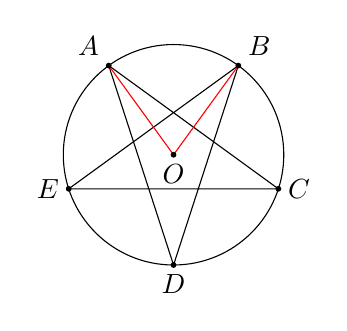
\begin{tikzpicture}[line join = round, line cap = round,>=stealth,scale=0.7]
	\coordinate[label = below:$O$] (O) at (0,0);
	\coordinate[label = below:$D$] (D) at (0,-2);
	\coordinate[label = right:$C$] (C) at (-18:2);
	\coordinate[label = left:$E$] (E) at (-162:2);
	\coordinate[label = above right:$B$] (B) at (54:2);
	\coordinate[label = above left:$A$] (A) at (126:2);
	\draw (O) circle (2 cm);	
	\draw (A)--(C) (A)--(D) (B)--(E) (B)--(D) (C)--(E);
	\draw[red] (O)--(A) (O)--(B);
	\foreach \x in {O,A,B,C,D,E} \fill[black] (\x) circle (1.5pt);	 
	\end{tikzpicture}}
	\loigiai{
	Các điểm $A$, $B$, $C$, $D$ và $E$ chia đường tròn thành 5 phần bằng nhau. \\
	Do đó $\widehat{AOB}=\dfrac{360^{\circ}}{5}=72^{\circ}$.\\
	Ta có $\widehat{AOB}=72^{\circ}$ là góc ở tâm chắn cung $\wideparen{AB}$.\\
	Suy ra cung nhỏ $\wideparen{AB}$ có sđ$\wideparen{AD}=72^{\circ}$ và cung lớn $\wideparen{AD}$ có sđ$\wideparen{DBA}=360^{\circ}-72^{\circ}=288^{\circ}$.
	}
\end{vd}
\begin{vd}%[9H3Y1-1]
	Cho hình vuông $ABCD$. Gọi $O$ là tâm đường tròn đi qua bốn điểm $A$, $B$, $C$, $D$.
	\begin{listEX}[2]
	\item Tính số đo góc ở tâm $\widehat{AOB}$, $\widehat{BOC}$.
	\item Tính số đo cung nhỏ $AB$, $CD$.
	\end{listEX}
	\loigiai
	{	\immini{
	\begin{enumerate}
	\item Gọi $O$ là giao điểm của $AC$ và $BD$. 
	Do $ABCD$ là hình vuông nên $OA=OB=OC=OD$. Vậy $O$ là tâm đường tròn đi qua $A$, $B$, $C$, $D$. $ABCD$ là hình vuông nên $AC\perp BD$, vậy $\widehat{AOB}=90^\circ$, $\widehat{BOC}=90^\circ$.
	\item Ta có $\widehat{AOB}=90^\circ\Rightarrow \text{sđ}\wideparen{AB}=90^\circ$; $\widehat{COD}=90^\circ\Rightarrow \text{sđ}\wideparen{CD}=90^\circ$.
	\end{enumerate}}{\begin{tikzpicture}[line join = round, line cap = round,>=stealth,scale=0.8]
	\tkzDefPoints{0/0/O}
	\tkzDefShiftPoint[O](-45:2){C}
	\tkzDefPointBy[symmetry = center O](C) \tkzGetPoint{A}
	\tkzDefShiftPoint[O](45:2){B}
	\tkzDefPointBy[symmetry = center O](B) \tkzGetPoint{D}
	\pgfresetboundingbox
	\tkzDrawCircle[radius](O,C)
	\tkzDrawSegments(A,C B,D A,B B,C C,D D,A)
	\tkzDrawPoints[fill=black,size=2pt](A,C,O,D)
	\tkzLabelPoints[left](A,D)
	\tkzLabelPoints[right](C,B)
	\tkzLabelPoints[below](O)
	\end{tikzpicture}}
	}
\end{vd}
\begin{vd}
	\immini{Biểu đồ hình quạt tròn ở hình bên biểu diễn kết quả thống kê (tính theo tỉ số phần trăm) chọn môn thể thao ưa thích nhất trong bốn môn: Cầu lông, Bóng bàn, Bóng chuyền, Bóng đá của $300$ học sinh khối lốp $9$ ở một trường trung học cơ sở (mỗi học sinh chỉ được chọn một môn thể thao khi được hỏi ý kiến). Tìm số đo của các góc ở tâm: $\widehat{AOB}; \widehat{COD}$; $\widehat{BOC}$; $\widehat{DOA}$.}
	{\begin{tikzpicture}[scale=0.7]
	\pie[text=inside]{25/\scriptsize Cầu lông,40/\scriptsize Bóng đá,20/\scriptsize Bóng\\ \scriptsize chuyền,15/\scriptsize Bóng bàn}
	\draw (0,3) node[above]{A};
	\draw (3,0) node[right]{B};
	\draw (-54:3) node[below right]{C};
	\draw (-127:3) node[below]{D};	
	\end{tikzpicture}}	
	\loigiai{
	\begin{itemize}
	\item Do số học sinh chọn môn Cầu lông chiếm $25\%$ số lượng học sinh nên số đo cung nhỏ $AB$ bằng $25\%$ số đo của cung cả đường tròn. \\
	Vì thế, $\text{sđ }\wideparen{AB}=\dfrac{25}{100}\cdot 360^{\circ}=90^{\circ}$. \\
	Vì số đo của cung nhỏ $AB$ bằng số đo của góc ở tâm $AOB$ chắn cung đó nên $\widehat{AOB}=90^{\circ}$.
	\item Do số học sinh chọn môn Bóng chuyển chiếm $20\%$ số lượng học sinh nên số đo cung nhỏ $AB$ bằng $20\%$ số đo của cung cả đường tròn.\\
	Vì thế, $\text{sđ }\wideparen{CD}=\dfrac{20}{100}\cdot 360^{\circ}=72^{\circ}$. \\
	Vì số đo của cung nhỏ $CD$ bằng số đo của góc ở tâm $COD$ chắn cung đó nên $\widehat{COD}=72^{\circ}$
	\item Do số học sinh chọn môn Bóng bàn chiếm $15\%$ số lượng học sinh nên số đo cung nhỏ $AB$ bằng $15\%$ số đo của cung cả đường tròn. \\
	Vì thế, $\text{sđ }\wideparen{BC}=\dfrac{15}{100}\cdot 360^{\circ}=54^{\circ}$. \\
	Vì số đo của cung nhỏ $AB$ bằng số đo của góc ở tâm $BOC$ chắn cung đó nên $\widehat{BOC}=54^{\circ}$.
	\item Do số học sinh chọn môn Bóng đá chiếm $40\%$ số lượng học sinh nên số đo cung nhỏ $AD$ bằng $40\%$ số đo của cung cả đường tròn. \\
	Vì thế, $\text{sđ }\wideparen{AD}=\dfrac{40}{100}\cdot 360^{\circ}=144^{\circ}$. \\
	Vì số đo của cung nhỏ $AD$ bằng số đo của góc ở tâm $AOD$ chắn cung đó nên $\widehat{AOD}=144^{\circ}$.
	\end{itemize}}
\end{vd}
\begin{vd}
	\immini{	 
	Tính số đo của các cung có các đầu mút là hai trong các điểm $A$, $B$, $C$ trong hình bên, biết rằng $ABC$ là tam giác vuông cân tại đỉnh $A$. }
	{
	\begin{tikzpicture}[declare function={r=1.5;ga=90;gb=180;gc=0;}]
	\path (0,0) coordinate (O) %tam
	(ga:r) coordinate (A)
	(gb:r) coordinate (B)
	(gc:r) coordinate (C);
	\draw[dashed,red] (O) circle (r);
	\draw (A)--(B)--(O)--(C)--cycle--(O);
	\foreach \t/\g in {A/90,B/180,C/0,O/-90}{
	\fill (\t) circle (1pt) node[shift={(\g:7pt)},font=\scriptsize]{$ \t $};	}
	\path pic[draw,angle radius=5pt]{right angle= B--A--C};
	\end{tikzpicture}}
	\loigiai{
	\begin{itemize}
	\item Ta thấy $\wideparen{AB}$ và $\wideparen{AC}$ là các cung nhỏ bị chắn bởi các góc ở tâm thứ tự là $\widehat{AOB}$ và $\widehat{AOC}$.\\ 
	Do tam giác $ABC$ vuông cân tại $A$ nên đường trung tuyến $AO$ cũng là đường cao, tức là $AO\perp BC$.\\
	Do đó $\widehat{AOB}=\widehat{AOC}=90^{\circ}$, suy ra $\text{sđ} \wideparen{AB}=\text{sđ} \wideparen{AC}=90^{\circ}$.
	\item $\widehat{ACB}$ là cung lớn có chung hai mút $A$, $B$ với cung nhỏ $AB$ nên
	$$\text {sđ} \wideparen{ACB}=360^{\circ}-\text {sđ} \wideparen{AB}=360^{\circ}-90^{\circ}=270^{\circ}.$$
	Tương tự, ta có $\text{sđ} \wideparen{ABC}=360^{\circ} -\text{sđ} \wideparen{AC} = 360^{\circ}-90^{\circ} = 270^{\circ}$.\\
	Ngoài ra còn có hai nửa đường tròn có chung hai mút $A$ và $B$, có số đo bằng $180^{\circ}$.
	\end{itemize}	}
\end{vd}
\begin{vd}
	Cho $C$ là điểm trên đường tròn $(O)$. Đường trung trực của đoạn $OC$ cắt $(O)$ tại $A$ và $B$. Tính số đo của các cung $\wideparen{ACB}$ và $\wideparen{ABC}$.
	\loigiai{
	\immini{	Vì $AB$ là trung trực của $OC$ nên $AO = AC$; $BO = BC$. Mà $OA = OB = R$. Do đó $AO=OB=BC=CA=R$.\\ Hay $\triangle AOC$ và $\triangle BOC$ là hai tam giác đều.\\ 
	Nên $\widehat {AOC}=\widehat {BOC}=60^\circ$ suy ra $\widehat {AOB}=120^\circ$.\\ 
	Vậy $\text{sđ }\wideparen {ACB} = 120^\circ$.\\
	Và $\text{sđ}\wideparen {ABC} = 360^\circ - \text{sđ}\wideparen {AC} = 360^\circ - 60^\circ = 300^\circ$.
	}
	{	\rule{1cm}{0pt}
	\begin{tikzpicture}[declare function={r=1.8;ga=90;gb=180;gc=0;}]
	\path (0,0) coordinate (O) %tam
	(gc:r) coordinate (C)
	($(O)!0.5!(C)$) coordinate (I)
	($(I)!2.5!-90:(O)$) coordinate (I1)
	($(I)!2.5!90:(O)$) coordinate (I2);
	\draw[name path = c1] (O) circle (r);
	\path[name path =d1] (I1)--(I2);
	\path[name intersections={of = c1 and d1,by={A,B}}];
	\draw (O)--(C) (A)--(C)--(B)--(O)--cycle--(B);
	\foreach \t/\g in {A/90,B/-90,C/0,O/180,I/-135}{
	\fill (\t) circle (1pt) node[shift={(\g:7pt)},font=\scriptsize]{$ \t $};	}
	\path pic[draw,angle radius=5pt]{right angle= A--I--C};
	\foreach \x/\y in {O/I,I/C}{
	\path (\x)--(\y) node[midway,sloped]{\tikz{\draw [shift={(-0.65pt,0)}](-90:1pt)--(90:1pt) [shift={(0.65pt,0)}](-90:1pt)--(90:1pt);}};	}
	\end{tikzpicture}}}
\end{vd}
%=========================
\begin{dang}{Tính số đo góc ở tâm, số đo cung tròn}
\end{dang}
\begin{vd}
	\immini
	{
	Một huấn luyện viên cho cầu thủ tập sút bóng vào cầu môn ${MN}$ (hình bên). Nếu bóng được đặt ở điểm ${X}$ thì $\widehat{{MXN}}$ gọi là góc sút từ vị trí ${X}$. Hãy so sánh các góc sút $\widehat{{MXN}}, \widehat{{MYN}}, \widehat{{MZN}}$.
	}
	{
	\begin{tikzpicture}[line join = round, line cap = round, >=stealth, font=\footnotesize, scale=.7]
	\path (0,0)coordinate (O) (2,0)coordinate (A) ;
	\draw[line width=0.4pt,black] let \p1=($(A)-(O)$) in (O) circle ({veclen(\x1,\y1)});
	\coordinate[label=right:$N$] (N) at ($(O)!1!-40:(A)$);
	\coordinate[label=left:$M$] (M) at ($(O)!1!-140:(A)$);
	\coordinate[label=right:$Z$] (Z) at ($(O)!1!40:(A)$);
	\coordinate[label=above:$Y$] (Y) at ($(O)!1!90:(A)$);
	\coordinate[label=left:$X$] (X) at ($(O)!1!160:(A)$);
	\draw (M)--(N)--(Z)--(M)--(X)--(N)--(Y)--(M);
	\foreach \diem in {M,N,Z,Y,Z} \fill[black](\diem)circle(1.5pt);
	\end{tikzpicture}
	}
	\loigiai{
	Ta thấy $\widehat{MXN}= \widehat{{MYN}}= \widehat{{MZN}} =\dfrac{1}{2}\text{sđ} \wideparen{MN}$. (các góc nội tiếp cùng chắn $\wideparen{MN}$)
	}
\end{vd}
\begin{vd}
	\immini{Tính số đo góc $MIN$ ở hình bên.}
	{\begin{tikzpicture}[line join = round, line cap = round,>=stealth,font=\footnotesize,scale=0.7]
	\def\r{2}
	\path 
	(0,0) coordinate (O)
	(\r,0) coordinate (X)
	($(O)!1!-10:(X)$) coordinate (M)
	($(O)!1!-120:(X)$) coordinate (N)
	($(O)!1!110:(X)$) coordinate (I)
	;
	\draw (O) circle(\r cm);
	\draw (M)--(I)--(N)--(O)--(M);
	\foreach \x/\g in {O/90,M/-10,N/-120,I/110}\fill[black] (\x) circle (1pt) ($(\x)+(\g:3mm)$) node{$\x$};
	%\draw (0,-2) node[below]{n};
	%\draw (-90:2) node[below]{m};
	\draw (-55:0.8) node[scale=0.8]{$100^\circ$};
	\foreach \a/\b/\c in {N/O/M,N/I/M}{\draw pic[draw,angle radius=2mm] {angle = \a--\b--\c};}
	\foreach \a/\b/\c in {N/O/M}{\draw pic[draw,angle radius=3.5mm] {angle = \a--\b--\c};}	
	\end{tikzpicture}}
	\loigiai{Xét đường tròn $(O)$ có
	$\widehat{MON}$ là góc ở tâm và $\widehat{MIN}$ là góc nội tiếp cùng chắn cung $MN$ nên
	$$
	\widehat{MIN}=\dfrac{1}{2}\widehat{MON}=\dfrac{1}{2}\cdot 100^{\circ}=50^{\circ}.
	$$
	Vậy $\widehat{MIN}=50^{\circ}$.}
\end{vd}
%----------------------------------
\begin{vd}
	Cho đường tròn $(O; R)$ và dây cung $AB=R$. Điểm $C$ thuộc cung lớn $AB$, $C$ khác $A$ và $B$. Tính số đo góc $ACB$.
	\loigiai{
	\immini{
	Ta có $OA=OB=AB$ nên tam giác $AOB$ đều nên $\widehat{BOC}=60^\circ$.\\
	Xét đường tròn $(O)$ có $\widehat{AOB}$ là góc ở tâm và $\widehat{ACB}$ là góc nội tiếp cùng chắn cung $AB$ nên
	$$
	\widehat{ACB}=\dfrac{1}{2}\widehat{AOB}=\dfrac{1}{2}\cdot 60^{\circ}=30^{\circ}.
	$$
	Vậy $\widehat{ACB}=30^{\circ}$.
	}
	{\begin{tikzpicture}[line join = round, line cap = round,>=stealth,font=\footnotesize,scale=0.7]
	\def\r{2}
	\path 
	(0,0) coordinate (O)
	(\r,0) coordinate (X)
	($(O)!1!30:(X)$) coordinate (A)
	($(O)!1!-30:(X)$) coordinate (B)
	($(O)!1!125:(X)$) coordinate (C)
	;
	\draw (O) circle(\r cm);
	\draw (A)--(C)--(B)--(A)--(O)--(B);
	\foreach \x/\g in {O/-170,A/30,B/-30,C/150}\fill[black] (\x) circle (1pt) ($(\x)+(\g:3.5mm)$) node{$\x$};
	\end{tikzpicture}} 
	}
\end{vd}
\begin{vd}
	\immini{Trong hình bên, gọi $I$ là giao điểm của $AD$ và $BC$. Chứng minh $IA\cdot ID=IB\cdot IC$.}
	{\begin{tikzpicture}[line join = round, line cap = round,>=stealth,font=\footnotesize,scale=0.7]
	\def\r{2}
	\path 
	(0,0) coordinate (O)
	(\r,0) coordinate (X)
	($(O)!1!-150:(X)$) coordinate (A)
	($(O)!1!-30:(X)$) coordinate (B)
	($(O)!1!140:(X)$) coordinate (C)
	($(O)!1!75:(X)$) coordinate (D);
	\draw (O) circle(\r cm);
	\draw (A)--(C)--(B)(A)--(D)--(B);
	\path (intersection of A--D and B--C) coordinate (I);
	\foreach \x/\g in {O/-90,A/-150,B/-30,C/140,D/75,I/-90}\fill[black] (\x) circle (1pt) ($(\x)+(\g:3mm)$) node{$\x$};
	%\draw (0,-2) node[below]{n};
	\draw (-90:2) node[below]{m};
	%\draw (45:0.7) node[scale=0.8]{$\alpha$};
	\foreach \a/\b/\c in {A/C/B,A/D/B}{\draw pic[draw,angle radius=2mm] {angle = \a--\b--\c};}	
	\end{tikzpicture}}
	\loigiai{
	Xét đường tròn $(O)$, ta có:\\
	- Các góc nội tiếp $ACB$ và $ADB$ cùng chắn cung $AB$ nên $\widehat{ACB}=\widehat{ADB}$ hay $\widehat{ACI}=\widehat{ADI}$.\\
	- Các góc nội tiếp $CAD$ và $CBD$ cùng chắn cung $CD$ nên $\widehat{CDA}=\widehat{CBD}$ hay $\widehat{CAI}=\widehat{DBI}$.\\
	Xét hai tam giác $IAC$ và $IBD$ có $\widehat{ACI}=\widehat{ADI}$ và $\widehat{CAI}=\widehat{DBI}$ nên 
	$\triangle IAC\backsim \triangle IBD$ (gg).\\
	Suy ra $\dfrac{IA}{IB}=\dfrac{IC}{ID}$ hay $IA\cdot ID=IB\cdot IC$.
	}
\end{vd}
%----------------------------------
\begin{vd}
	\immini{Tìm số đo cung $ADB$ và số đo góc $ACB$ ở hình bên.}
	{\begin{tikzpicture}[line join = round, line cap = round,>=stealth,font=\footnotesize,scale=0.7]
	\def\r{2}
	\path 
	(0,0) coordinate (O)
	(\r,0) coordinate (X)
	($(O)!1!140:(X)$) coordinate (A)
	($(O)!1!10:(X)$) coordinate (B)
	($(O)!1!80:(X)$) coordinate (C)
	($(O)!1!-75:(X)$) coordinate (D);
	\draw (O) circle(\r cm);
	\draw (A)--(C)--(B)--(D)--(A)--(O)--(B)--(A);
	\foreach \x/\g in {O/-90,A/160,B/30,C/80,D/-75}{\draw[black] (\x) circle (1pt) ($(\x)+(\g:3mm)$) node{$\x$};}
	\draw (75:0.55) node[scale=0.8]{$130^\circ$};
	\foreach \a/\b/\c in {B/O/A}{\draw pic[draw,angle radius=2mm] {angle = \a--\b--\c};}	
	\end{tikzpicture}}
	\loigiai{Xét đường tròn $(O)$, ta có:
	$$
	\begin{aligned}
	\text{sđ } \wideparen{ADB}&=360^{\circ}-\text{sđ } \wideparen{ACB}\\
	&=360^{\circ}-\widehat{AOB}=360^{\circ}-130^{\circ}=230^{\circ}.
	\end{aligned}
	$$
	Vì $\widehat{ACB}$ là góc nội tiếp chắn cung $ADB$ nên
	$$
	\widehat{ACB}=\dfrac{1}{2}\text{sđ } \wideparen{ADB}=\dfrac{1}{2}\cdot 230^{\circ}=115^{\circ}.
	$$
	Vậy sđ $\widehat{ADB}=230^{\circ}; \widehat{ACB}=115^{\circ}$.}
\end{vd}
\begin{vd}
	Cho ba điểm ${A}$, ${B}$, ${C}$ nằm trên đường tròn $({O})$ sao cho $\widehat{{AOB}}=50^{\circ}$, $\widehat{{BOC}}=30^{\circ}$, điểm ${B}$ thuộc cung nhỏ ${AC}$. Gọi ${M}$, ${N}$ lần lượt là hai điểm trên hai cung nhỏ $\wideparen{{AB}}, \wideparen{{AC}}$ và chia mỗi cung đó thành hai cung bằng nhau. Tìm số đo các góc sau:
	\begin{listEX}[2]
	\item $\widehat{{BCA}}$, $\widehat{{BAC}}$;
	\item $\widehat{{MBA}}$, $\widehat{{BAN}}$.
	\end{listEX}
	\loigiai{
	\immini{\vspace*{-2mm}
	\begin{listEX}[1]
	\item Ta có $\widehat{BCA}=\dfrac{1}{2}\widehat{AOB}=\dfrac{1}{2}\cdot 50^\circ=25^\circ.$ (góc nội tiếp và góc ở tâm cùng chắn cùng $\wideparen{AB}$).\\
	Ta có $\widehat{BAC}=\dfrac{1}{2}\widehat{BOC}=\dfrac{1}{2}\cdot 30^\circ=15^\circ.$ (góc nội tiếp và góc ở tâm cùng chắn cùng $\wideparen{BC}$)
	\item Ta có $\widehat{MBA}=\dfrac{1}{2}\widehat{MOA}=\dfrac{1}{2}\cdot 25^\circ=12{,}5^\circ.$ (góc nội tiếp và góc ở tâm cùng chắn cùng $\wideparen{MA}$)
	\\
	Ta có $\widehat{BAN}=\dfrac{1}{2}\widehat{BON}=\dfrac{1}{2}\cdot 15^\circ=7{,}5^\circ.$ (góc nội tiếp và góc ở tâm cùng chắn cùng $\wideparen{BN}$)
	\end{listEX}}{
	\begin{tikzpicture}[line join = round, line cap = round, >=stealth, font=\small, scale=1]
	\path (0,0)coordinate[label=below:$O$](O) (2,0)coordinate[label=right:$A$](A) ;
	\draw[line width=0.4pt,black] let \p1=($(A)-(O)$) in (O) circle ({veclen(\x1,\y1)});
	\coordinate[label=above right:$B$] (B) at ($(O)!1!50:(A)$);
	\coordinate[label=above :$C$] (C) at ($(O)!1!30:(B)$);
	\coordinate[label=right :$M$] (M) at ($(O)!1!25:(A)$);
	\coordinate[label=above :$N$] (N) at ($(O)!1!15:(B)$);
	\draw (A)--(O)--(B) (O)--(C);
	\foreach \diem in {A,B,C,O,M,N} \fill[black](\diem)circle(1.5pt);
	\draw pic[angle radius=6mm,draw=black,"${\small 30^\circ}$",angle eccentricity=1.5] {angle = B--O--C};
	\draw pic[angle radius=5.5mm,draw=black,angle eccentricity=1.5] {angle = B--O--C};
	\draw pic[angle radius=5mm,draw=black,"$50^\circ$",angle eccentricity=1.5] {angle = A--O--B};
	\end{tikzpicture}
	}
	}
\end{vd}
\begin{vd}
	\immini
	{
	Cho $AB$ và $CD$ là hai đường kính vuông góc của đường tròn $(O)$. Gọi $M$, $N$ là hai điểm lần lượt trên hai cung nhỏ $\wideparen{AC}$, $\wideparen{BC}$ và chia mỗi cung đó thành hai cung bằng nhau. Tìn số đo các góc sau:
	\begin{listEX}[1]
	\item $\widehat{ACB}$, $\widehat{ADC}$;
	\item $\widehat{ADM}$, $\widehat{NCB}$.
	\end{listEX}
	}
	{
	\begin{tikzpicture}[line join = round, line cap = round, >=stealth, font=\small, scale=0.8]
	\path (0,0)coordinate[label=below left:$O$](O) (-2,0)coordinate[label=left:$A$](A)
	(2,0)coordinate[label=right:$B$](B)
	(0,2)coordinate[label=above:$C$](C)
	(0,-2)coordinate[label=below:$D$](D);
	\draw[line width=0.4pt,black] let \p1=($(A)-(O)$) in (O) circle ({veclen(\x1,\y1)});
	\coordinate[label=above right:$N$] (N) at ($(O)!1!45:(B)$);
	\coordinate[label=above left:$M$] (M) at ($(O)!1!45:(C)$);
	\draw pic[angle radius=2mm,draw=blue,angle eccentricity=1.5] {right angle = B--O--C};
	\draw (A)--(B) (D)--(C)--(B)--(N)--(C)--(A)--(D)--(M)--(B) (M)--(A)--(N);
	\foreach \diem in {A,O,B,C,D,M,N} \fill[black](\diem)circle(1.5pt);
	\end{tikzpicture}
	}
	\loigiai
	{
	\begin{listEX}[1]
	\item Ta có $\widehat{{ACB}}$ là góc nội tiếp chắn nửa đường tròn$, $suy ra $\widehat{{ACB}}=90^{\circ}$.\\
	Ta có $\widehat{{ADC}}$ và $\widehat{{AOC}}$ lần lượt là góc nội tiếp và góc ở tâm cùng chắn cung ${AC}$, suy ra $$\widehat{{ADC}}=\dfrac{\widehat{{AOC}}}{2}=\dfrac{90^{\circ}}{2}=45^{\circ}.$$
	\item Do hai đường kính $AB$ và $CD$ vuông góc với nhau tại tâm $O$ của $(O)$ nên $\widehat{AOC}=\widehat{COB}=\widehat{BOD}=\widehat{DOA}=90^{\circ}$ suy ra $\text{sđ}\wideparen{AC}=\text{sđ}\wideparen{CB}=\text{sđ}\wideparen{BD}=\text{sđ}\wideparen{DA}=90^{\circ}.$
	\\
	Vì $M$, $N$ lần lượt chia $\wideparen{{AC}}$, $\wideparen{{CB}}$ thành hai cung có số đo bằng nhau nên
	$$ \text{sđ}\wideparen{AM}=\text{sđ}\wideparen{MC}=\text{sđ}\dfrac{\wideparen{AC}}{2}=45^{\circ} , \text{sđ}\wideparen{CN}=\text{sđ}\wideparen{NB}=\text{sđ}\dfrac{\wideparen{CB}}{2}=45^{\circ}.$$
	\\
	Ta có $\widehat{{ADM}}$ là góc nội tiếp chắn cung ${AM}$, suy ra
	$$
	\widehat{{ADM}}=\dfrac{\text{sđ} \wideparen{{AM}}}{2}=\dfrac{45^{\circ}}{2}=22{,}5^{\circ}.
	$$
	Ta có $\widehat{{NCB}}$ là góc nội tiếp chắn cung ${NB}$, suy ra
	$$
	\widehat{{NCB}}=\dfrac{\text{sđ} \widehat{{BN}}}{2}=\dfrac{45^{\circ}}{2}=22{,}5^{\circ}.
	$$
	\end{listEX}
	}
\end{vd}
\begin{vd}%[9H3B2-1]
	Cho $\triangle ABC$ nội tiếp đường tròn $(O)$. Các cung nhỏ $AB$, $BC$, $AC$ có số đo lần lượt là $x+10^\circ$, $x+20^\circ$, $x+30^\circ$. Tính số đo các góc của tam giác $ABC$.
	\loigiai{
	\immini{
	Ta có $\text{sđ}\wideparen{AB}+\text{sđ}\wideparen{BC}+\text{sđ}\wideparen{AC}=360^\circ$ nên $x+10^\circ+x+20^\circ+x+30^\circ=360^\circ$ $\Rightarrow x=100^\circ$. Do đó, $\text{sđ}\wideparen{AB}=110^\circ$, $\text{sđ}\wideparen{BC}=120^\circ$, $\text{sđ}\wideparen{AC}=130^\circ$. Vậy $\widehat{C}=55^\circ$, $\widehat{A}=60^\circ$, $\widehat{B}=65^\circ$.	}{
	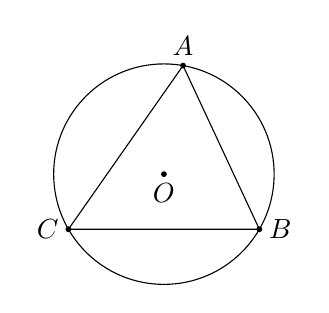
\begin{tikzpicture}[line join = round, line cap = round,>=stealth,scale=0.7]
	\coordinate[label = below:$O$] (O) at (0,0);
	\coordinate[label = above:$A$] (A) at (80:2);
	\coordinate[label = right:$B$] (B) at (-30:2);
	\coordinate[label = left:$C$] (C) at (-150:2);
	\draw (O) circle (2 cm);	
	\draw (A)--(B)--(C)--cycle;
	\foreach \x in {O,A,B,C} \fill[black] (\x) circle (1.5pt);	
	\end{tikzpicture}
	}
	}
\end{vd}
\begin{vd}%[9H3B2-1]
	\immini{Cho hình bên, biết $BD$ là đường kính của $(O)$, $\widehat{BAC}=40^\circ$. Tính số đo của góc $\widehat{CBD}$.}{\begin{tikzpicture}[line join = round, line cap = round,>=stealth,
	font=\footnotesize,scale=.8]
	\tkzDefPoints{0/0/B}
	\coordinate (C) at ($(B)+(4,0)$);
	\tkzDefShiftPoint[B](75:3){A}
	\tkzDrawPolygon(A,B,C)
	\tkzCircumCenter(A,B,C) \tkzGetPoint{O}
	%
	\tkzDefPointBy[symmetry = center O](B)
	\tkzGetPoint{D}
	\draw let \p1=($(B)-(O)$) in (O) circle ({veclen(\x1,\y1)});
	\tkzDrawPoints[fill=black](A,B,C,O,D)
	\tkzDrawSegments(B,D C,D)
	\tkzLabelPoints[below left](B)
	\tkzLabelPoints[below right](C)
	\tkzLabelPoints[above](A) \tkzLabelPoints[right](D)
	\tkzLabelPoints[below](O)
	\end{tikzpicture}}
	\loigiai{
	$\widehat{BAC}=\widehat{BDC}$ (hệ quả góc nội tiếp) nên $\widehat{40^\circ}$; $BD$ là đường kính nên $\widehat{BCD}=90^\circ$ nên $\triangle BCD$ vuông. Do đó $\widehat{CBD}+\widehat{BDC}=90^\circ$. Vậy $\widehat{CBD}=50^\circ$.
	}
\end{vd}
\begin{vd}%[9H3K2-1]
	Cho $\triangle ABC$ nhọn có $\widehat{BAC}=60^\circ$. Vẽ đường tròn đường kính $BC$ tâm $O$ cắt $AB$, $AC$ tại $D$ và $E$. Chứng minh $\widehat{ODE}=60^\circ$.
	\loigiai{\immini{
	$\widehat{BDC}=90^\circ$ (góc nội tiếp chắn nửa đường tròn) nên\\ $\widehat{ADC}=90^\circ$ do đó $\triangle ADC$ vuông tại $D$. Ta có $\widehat{DAC}+\widehat{ACD}=90^\circ$ $\Rightarrow \widehat{ACD}=30^\circ$.
	Mặt khác, $\widehat{DCE}=\dfrac{1}{2}\widehat{DOE}$ (hệ quả góc nội tiếp) nên $\widehat{DOE}=60^\circ$.\\Ta có $OD=OE$ (bán kính) do đó $\triangle ODE$ đều. Vậy $\widehat{ODE}=60^\circ$.}{\begin{tikzpicture}[line join = round, line cap = round,>=stealth,
	font=\footnotesize,scale=0.8]
	\tkzDefPoints{0/0/B}
	\coordinate (C) at ($(B)+(4,0)$);
	\tkzDefShiftPoint[B](60:4){A}
	\tkzDrawPolygon(A,B,C)
	\coordinate (O) at ($(C)!0.5!(B)$);
	\tkzDrawCircle[black](O,B)
	\tkzInterLC(A,B)(O,C)
	\tkzGetPoints{D}{}
	\tkzInterLC(A,C)(O,B)
	\tkzGetPoints{}{E}
	%
	\tkzDrawPoints[fill=black](A,B,C,O,D,E)
	\tkzDrawSegments(D,C O,E O,D D,E)
	\tkzLabelPoints[below left](B)
	\tkzLabelPoints[below right](C)
	\tkzLabelPoints[above](A)
	\tkzLabelPoints[above left](D)
	\tkzLabelPoints[below](O)
	\tkzLabelPoints[above right](E)
	\end{tikzpicture}}
	}
\end{vd}
%===========================
\begin{dang}{Chứng minh ba điểm thẳng hàng. Hai đường thẳng vuông góc}
%\begin{itemize}
%	\item Chứng minh ba điểm thẳng hàng:
%	\begin{itemize}
%	\item Góc nội tiếp bằng $90^\circ$ thì chắn nửa đường tròn.
%	\item Hai đầu đường kính và tâm đường tròn thẳng hàng. 
%	\end{itemize}	
%	\item Chứng minh hai đường thẳng vuông góc
%	\begin{itemize}
%	\item Sử dụng định lí và hệ quả góc nội tiếp.
%	\item Sử dụng tính chất tam giác vuông.
%	\end{itemize}	
%\end{itemize}
\end{dang}
\begin{vd}%[9H3K2-1]
	Cho $\triangle ABC$ nhọn có $\widehat{BAC}=45^\circ$ nội tiếp đường tròn $(O)$. Các đường cao $BH$, $CK$ cắt đường tròn $(O)$ tại $D$, $E$. Chứng minh $D$, $O$, $E$ thẳng hàng.
	\loigiai{\immini{
	Ta có $BH\perp AC$ nên $\triangle ABH$ vuông tại $H$. Mà $\widehat{BAH}=45^\circ$ nên $\widehat{ABH}=45^\circ$.Mặt khác $\widehat{ABD}=\widehat{ACD}$ (góc nội tiếp cùng chắn cung $\wideparen{AD}$)	 nên $\widehat{ACD}=45^\circ$.\tagEX{1} $CK\perp AB$ nên $\triangle ACK$ vuông tại $K$. Mà $\widehat{CAK}=45^\circ$ nên $\widehat{ACK}=45^\circ$. \tagEX{2}
	Từ (1) và (2) ta có $\widehat{DCE}=90^\circ$ nên $DE$ là đường kính. Vậy $D$, $O$, $E$ thẳng hàng.
	}{
	\begin{tikzpicture}[font=\footnotesize, line join=round, line cap=round, >=stealth,scale=0.7]
	\tkzDefPoints{0/0/B,4/0/C}
	\tkzDefTriangle[two angles = 75 and 60](B,C)
	\tkzGetPoint{A}
	\draw (A)--(B)--(C)--cycle;
	\tkzCircumCenter(A,B,C)
	\tkzGetPoint{O}
	\coordinate (K) at ($(A)!(C)!(B)$);
	\coordinate (H) at ($(A)!(B)!(C)$);
	\tkzInterLC(B,H)(O,A)\tkzGetPoints{}{D}
	\tkzInterLC(C,K)(O,A)\tkzGetPoints{E}{}
	\draw let \p1=($(A)-(O)$) in (O) circle ({veclen(\x1,\y1)});
	\tkzMarkRightAngle[](B,K,C)
	\tkzMarkRightAngle[](B,H,C)
	\tkzDrawPoints[fill=black](A,B,C,H,K,D,E,O)
	\tkzDrawSegments[](B,D C,E K,C B,H)
	\tkzDrawSegments[dashed](D,E)
	\tkzLabelPoints[above](A)
	\tkzLabelPoints[left](B)
	\tkzLabelPoints[right](C)
	\tkzLabelPoints[above right](K)
	\tkzLabelPoints[right](H)
	\tkzLabelPoints[below](O)
	\tkzLabelPoints[right](D)
	\tkzLabelPoints[left](E)
	\end{tikzpicture}}
	}
\end{vd}
\begin{vd}%[9H3K2-1]
	Hai đường tròn $(O)$ và $(O')$ cắt nhau tại $A$ và $B$ sao cho $\widehat{OAO'}=90^\circ$, lấy điểm $C$ thuộc $(O')$ và ở bên ngoài đường tròn $(O)$. Kẻ các tia $CA$, $CB$ cắt đường tròn $(O)$ tại $D$, $E$. Chứng minh rằng $D$, $O$, $E$ thẳng hàng.
	\loigiai{\immini{
	\begin{itemize}
	\item Xét $(O)$ ta có $\widehat{AEB}=\dfrac{1}{2}\widehat{AOB}$. \hfill(1)
	\item Xét $(O')$ ta có $\widehat{ACB}=\dfrac{1}{2}\widehat{AO'B}$. \hfill(2)
	\item Từ (1) và (2) ta có $\widehat{AEB}+\widehat{ACB}=\dfrac{1}{2}\cdot \left(\widehat{AOB}+\widehat{AO'B}\right)=90^\circ$. Nên $\widehat{EAC}=90^\circ$, do đó $\widehat{DAE}=90^\circ$. Vậy $D$, $E$, $O$ thẳng hàng.
	\end{itemize}	}{\begin{tikzpicture}[scale=0.5, font=\footnotesize, line join=round, line cap=round, >=stealth]
	\tikzset{label style/.style={font=\footnotesize}}
	\tkzDefPoint(0,0){O} \tkzDefPoint(5,0){O'}
	\draw (O) circle (4cm);
	\draw (O') circle (3cm);
	\tkzInterCC[R](O,4 )(O',3 ) \tkzGetPoints{A}{B}
	\tkzDrawPolygon(A,O,O')
	\tkzDefPointBy[rotation = center O' angle -110](A)
	\tkzGetPoint{C}
	\tkzInterLC(C,A)(O,A) \tkzGetPoints{}{D}
	\tkzInterLC(C,B)(O,A) \tkzGetPoints{E}{}
	\tkzDrawPoints[fill=black](O,O',A,B,C,D,E)
	\tkzDrawSegments[](C,E D,C O,B O',B)
	\tkzDrawSegments[dashed](D,E)
	\tkzMarkRightAngles[](O,A,O')
	\tkzLabelPoints[above](A,D)
	\tkzLabelPoints[left](O)
	\tkzLabelPoints[right](O',C)
	\tkzLabelPoints[below](E,B)
	\end{tikzpicture}}	
	}
\end{vd}
\begin{vd}%[9H3K2-1]
	Cho đường tròn $(O)$ có dây cung $AC$ và $BD$ vuông góc với nhau tại $I$. Gọi $M$ là trung điểm của $BC$. Chứng minh $IM\perp AD$.
	\loigiai{
	\immini{
	Gọi $N$ là giao điểm của $MI$ và $AD$; $AC\perp BD$ tại $I$ nên $\triangle BCI$ vuông tại $I$.\\
	Mà $MB=MC$ $\Rightarrow MI=MB$ (tính chất đường trung tuyến của tam giác vuông) nên $\triangle MBI$ cân.\\
	Do đó, $\widehat{MIB}=\widehat{MBI}$ mà $\widehat{NID}=\widehat{BIM}$ ( đối đỉnh) do đó $\widehat{MBI}=\widehat{NID}$. \tagEX{1}
	Ta có $\widehat{BDA}=\widehat{BCA}$ (góc nội tiếp cùng chắn cung $\wideparen{AB}$). \tagEX{2}
	Mà $\widehat{BCA}+\widehat{MBI}=90^\circ$ ($\triangle BCI$ vuông tại $I$) nên từ (1) và (2) ta có $\widehat{NID}+\widehat{BDA}=90^\circ$ hay $\triangle IND$ vuông tại $N$. Vậy $MN\perp AD$.
	}{\begin{tikzpicture}[scale=0.8, font=\footnotesize, line join=round, line cap=round, >=stealth]
	\tikzset{label style/.style={font=\footnotesize}}
	\tkzInit[xmin=-3.5,xmax=3.5,ymin=-3.5,ymax=3]
	\tkzClip
	\tkzDefPoint(-3,0){A} \tkzDefPoint(3,0){C} \tkzDefPoint(-2,2){B}
	\tkzCircumCenter(A,B,C)
	\tkzGetPoint{O}
	\tkzCircumCenter(A,B,C)
	\coordinate (I) at ($(A)!(B)!(C)$);
	\tkzInterLC(B,I)(O,A) \tkzGetPoints{}{D}
	\tkzDefMidPoint(C,B)
	\tkzGetPoint{M}
	\tkzInterLL(M,I)(A,D)
	\tkzGetPoint{N}
	\draw let \p1=($(A)-(O)$) in (O) circle ({veclen(\x1,\y1)});'l;
	\tkzDrawSegments[](A,C B,C B,D A,D M,N C,I)
	\tkzMarkSegments[mark=|,size=2,thin](B,M M,C)
	\tkzDrawPoints[fill=black](O,A,B,C,D,I,M,N)
	\tkzLabelPoints[above](B)
	\tkzLabelPoints[below](O,D)
	\tkzLabelPoints[below right](N)
	\tkzLabelPoints[left](A)
	\tkzLabelPoints[above left](I)
	\tkzLabelPoints[right](C,M)
	\end{tikzpicture}}	
	}
\end{vd}	
\begin{vd}%[9H3K2-1]
	Cho tam giác $ABC$ nội tiếp đường tròn $(O)$. Tia phân giác góc $BAC$ cắt đường tròn $(O)$ tại $D$. Đường tròn tâm $D$, bán kính $DB$ cắt đường thẳng $AB$ tại $Q$ (khác $B$), cắt đường thẳng $AC$ tại $P$ (khác $C$). Chứng minh $AO\perp PQ$.
	\loigiai{\immini{
	Gọi $I$ và $E$ là giao điểm của $AO$ với đường tròn tâm $O$ và $PQ$. Ta có $\widehat{QBC}=\widehat{CPQ}$. Suy ra $\widehat{ABC}=\widehat{APQ}$ mà $\widehat{ABC}=\widehat{AIC}$ nên $\widehat{APQ}=\widehat{AIC}$. Do $\widehat{AIC}+\widehat{EAC}=90^\circ$ nên $\widehat{AEP}=90^\circ$.\\
	Vậy $AO\perp PQ$.
	}{\begin{tikzpicture}[scale=0.9, font=\footnotesize, line join=round, line cap=round, >=stealth]
	\tkzDefPoints{0/0/B,4/0/C}
	\tkzDefTriangle[two angles = 75 and 50](B,C)
	\tkzGetPoint{A}
	\draw (A)--(B)--(C)--cycle;
	\tkzCircumCenter(A,B,C)
	\tkzGetPoint{O}
	\tkzDefLine[bisector](B,A,C) \tkzGetPoint{Tempt}
	\tkzInterLL(A,Tempt)(B,C) \tkzGetPoint{V}
	\tkzInterLC(A,V)(O,A) \tkzGetPoints{}{D}
	\tkzInterLC(A,O)(O,A) \tkzGetPoints{}{I}
	\tkzDrawCircle[black](O,A)
	\tkzDrawCircle[black](D,B)
	\tkzGetPoint{O'}
	\tkzInterLC(A,B)(D,B) \tkzGetPoints{}{Q}
	\tkzInterLC(A,C)(D,B) \tkzGetPoints{}{P}
	\tkzInterLL(A,O)(P,Q)
	\tkzGetPoint{E}
	\tkzDrawSegments[](A,D D,B D,C A,I I,C P,Q A,Q)
	\tkzDrawPoints[fill=black](A,B,C,D,I,Q,P,E,O)
	\tkzLabelPoints[above](A)
	\tkzLabelPoints[below](D,I)
	\tkzLabelPoints[below right](E)
	\tkzLabelPoints[left](B,Q)
	\tkzLabelPoints[right](C,P,O)
	\end{tikzpicture}}
	}
\end{vd}
%==============================
\begin{dang}{Chứng minh một số hệ thức hình học}
\end{dang}
\begin{vd}%[9H3B2-1]
	Cho $\triangle ABC$ nhọn nội tiếp đường tròn $(O)$ có đường cao $AH$. Kẻ đường kính $AD$.
	\begin{listEX}[2]
	\item Tính góc $\widehat{ACD}$.
	\item Chứng minh $\widehat{BAH}=\widehat{OAC}$.
	\end{listEX}
	\loigiai{\immini{
	\begin{enumerate}
	\item $AD$ là đường kính của $(O)$ nên $\widehat{ACD}=90^\circ$ (góc nội tiếp chắn nửa đường tròn).
	\item $\widehat{ACD}=90^\circ$ nên $\triangle ACD$ vuông tại $C$ do đó,\\ $\widehat{DAC}+\widehat{ADC}=90^\circ$. \tagEX{1}
	$AH$ là đường cao nên $\triangle ABH$ vuông tại $H$ do đó, $\widehat{BAH}+\widehat{ABH}=90^\circ$. \tagEX{2}
	Mặt khác, $\widehat{ABH}=\widehat{ADC}$ (góc nội tiếp cùng chắn cung $\wideparen{AC}$). Từ (1) và (2) ta có $\widehat{DAC}=\widehat{BAH}$.
	\end{enumerate}	}{\begin{tikzpicture}[line join = round, line cap = round,>=stealth,
	font=\footnotesize,scale=0.9]
	\tkzDefPoints{0/0/B}
	\coordinate (C) at ($(B)+(4,0)$);
	\tkzDefShiftPoint[B](70:3){A}
	\tkzDrawPolygon(A,B,C)
	\tkzCircumCenter(A,B,C) \tkzGetPoint{O}
	%
	\tkzDefPointBy[projection= onto C--B](A)
	\tkzGetPoint{H}
	\tkzDefPointBy[symmetry = center O](A)
	\tkzGetPoint{D}
	\draw let \p1=($(A)-(O)$) in (O) circle ({veclen(\x1,\y1)});
	\tkzMarkRightAngle[size=0.2,fill=gray!50](A,H,C)
	\tkzDrawPoints[fill=black](A,B,C,O,H,D)
	\tkzDrawSegments(A,H A,D C,D)
	\tkzLabelPoints[below left](B)
	\tkzLabelPoints[below right](C)
	\tkzLabelPoints[above](A)
	\tkzLabelPoints[below](O,H,D)
	\end{tikzpicture}}
	}
\end{vd}
\begin{vd}%[9H3B2-2]
	Cho đường tròn $(O)$ đường kính $AB$ và một dây cung $AP$. Tia $AP$ cắt tiếp tuyến tại $B$ của đường tròn ở $T$. Chứng minh
	\begin{listEX}[2]
	\item $\widehat{AOP}=2\cdot \widehat{ATB}$.
	\item $\widehat{APO}=\widehat{PBT}$.
	\end{listEX}
	\loigiai{\immini{
	\begin{enumerate}
	\item Ta có $\widehat{ATB}=\widehat{B_1}$ (cùng phụ với $\widehat{B_2}$). Mà $\widehat{B_1}=\dfrac{1}{2}\widehat{AOP}$ (hệ quả). Nên $\widehat{ATB}=\dfrac{1}{2}\widehat{AOP}$ hay $\widehat{AOP}=2\cdot \widehat{ATB}$.
	\item $AO=PO$ nên $\triangle AOP$ cân tại $O$ suy ra $\widehat{PAO}=\widehat{OPA}$. Mà $\widehat{PAO}=\widehat{PBT}$ (cùng phụ với $\widehat{B_1}$), suy ra $\widehat{OPA}=\widehat{PBT}$.
	\end{enumerate}	}{\begin{tikzpicture}[line join = round, line cap = round,>=stealth,
	font=\footnotesize,scale=1]	
	\tkzDefPoints{0/0/O,-2/0/A,2/0/B}
	\tkzDrawCircle(O,A)
	\tkzDefPointBy[rotation = center O angle 55](B)\tkzGetPoint{P}
	\tkzDefTangent[at=B](O) \tkzGetPoint{t}
	\tkzInterLL(A,P)(B,t)
	\tkzGetPoint{T}
	\draw let \p1=($(A)-(O)$) in (O) circle ({veclen(\x1,\y1)}); 
	\tkzLabelAngles[pos=-0.5,rotate=30](O,B,P){\small$1$}
	\tkzLabelAngles[pos=-0.5,rotate=30](P,B,T){\small$2$}
	\tkzDrawPoints[fill=black](A,B,O,P,T)
	\tkzDrawSegments(A,B A,T B,P B,T O,P)
	\tkzLabelPoints[above](P,T)
	\tkzLabelPoints[right](B)
	\tkzLabelPoints[left](A)
	\tkzLabelPoints[below](O)
	\end{tikzpicture}}
	}
\end{vd}
\begin{vd}%[9H3K2-1]
	Cho $\triangle ABC$ nhọn nội tiếp đường tròn $(O)$. Đường cao $AD$, $BE$ của $\triangle ABC$ cắt nhau tại $H$. $AD$ cắt đường tròn tại $I$. Chứng minh $DH=DI$.
	\loigiai{\immini{
	Ta có $\widehat{IAC}=\widehat{CBI}$ (góc nội tiếp cùng chắn cung $\wideparen{CI}$); $\widehat{IAC}=\widehat{EBC}$ (phụ với góc $C$).
	\\ Do đó $\widehat{IBC}=\widehat{EBC}$.
	\\ Xét $\triangle HBI$ có $BD$ là đường phân giác; $BD$ là đường cao ($AD\perp BC$). Nên $\triangle HBI$ cân tại $B$, do đó $BD$ là trung tuyến.
	\\ Vậy $DH=DI$.
	}{\begin{tikzpicture}[scale=1, font=\footnotesize, line join=round, line cap=round, >=stealth]
	\tkzDefPoints{0/0/B,4/0/C}
	\tkzDefTriangle[two angles = 75 and 50](B,C)
	\tkzGetPoint{A}
	\draw (A)--(B)--(C)--cycle;
	\tkzCircumCenter(A,B,C)
	\tkzGetPoint{O}
	\coordinate (D) at ($(B)!(A)!(C)$);
	\tkzInterLC(A,D)(O,A) \tkzGetPoints{}{I}
	\coordinate (E) at ($(A)!(B)!(C)$);
	\tkzInterLL(A,D)(B,E)
	\tkzGetPoint{H}
	\tkzDrawCircle[radius,black](O,A) 
	\tkzDrawSegments[](A,C B,C B,D A,I B,I A,D B,E)
	\tkzMarkRightAngle(A,D,B)
	\tkzMarkRightAngle(B,E,A)
	\tkzDrawPoints[fill=black](O,A,B,C,D,I,E,H)
	\tkzLabelPoints[above](A)
	\tkzLabelPoints[above right](D)
	\tkzLabelPoints[below](O,I)
	\tkzLabelPoints[left](B)
	\tkzLabelPoints[right](C,H,E)
	\end{tikzpicture}}	
	}
\end{vd}
\begin{vd}%[9H3G2-1]
	Cho $\triangle ABC$ đều nội tiếp đường tròn $(O)$. Lấy $M$ nằm trên cung $BC$. Chứng minh rằng $AM=BM+CM$.
	\loigiai{\immini{
	Trên dây $MA$ lấy $N$ sao cho $MN=BM$. \hfill $(1)$\\
	Ta có $\widehat{BMN}=\widehat{BCA}$ (góc nội tiếp chắn cung $\wideparen{AB}$) nên $\widehat{BMN}=60^\circ$ (do $\widehat{BCA}=60^\circ$).
	\\ $\triangle BMN$ có $MN=BM$, $\widehat{BMN}=60^\circ$ nên $\triangle BMN$ đều, do đó $BN=BM$, $\widehat{MBN}=60^\circ$.
	\\ Ta có $\widehat{B_1}+\widehat{B_2}=60^\circ$ (do $\triangle ABC$ đều); $\widehat{B_2}+\widehat{B_3}=60^\circ$ (do $\triangle BMN$ đều), nên $\widehat{B_1}=\widehat{B_3}$.
	\\ Xét $\triangle ABN$ và $\triangle CBM$ có
	\\$NB=MB$ (chứng minh trên); \hfill $(2)$\\
	$\widehat{B_1}=\widehat{B_3}$ (chứng minh trên); $AB=CB
	$ ($\triangle ABC$ đều) nên $\triangle ABN=\triangle CBM$ (c.g.c). Do đó $AN=CM$. \hfill $(3)$\\
	\\ Từ (1) và (2) suy ra $AM=BM+CM$. 	
	}{\begin{tikzpicture}[scale=1.2, font=\footnotesize, line join=round, line cap=round, >=stealth]
	\tkzDefPoints{0/0/B,4/0/C}
	\tkzDefTriangle[two angles = 60 and 60](B,C)
	\tkzGetPoint{A}
	\draw (A)--(B)--(C)--cycle;
	\tkzCircumCenter(A,B,C)
	\tkzGetPoint{O}
	\tkzDefPointBy[rotation = center O angle 150](A)
	\tkzGetPoint{M}
	\tkzInterLC(A,M)(M,B) \tkzGetPoints{N}{}
	\tkzDrawCircle[radius,black](O,A) 
	\tkzDrawSegments[](A,C B,C B,M M,C A,M B,N)
	\tkzMarkAngle[size=0.75](N,B,A)
	\tkzMarkAngle[size=0.75](C,B,N)
	\tkzMarkAngle[size=0.75](M,B,C)
	\tkzLabelAngles[pos=0.5](N,B,A){\tiny$1$}
	\tkzLabelAngles[pos=0.5](C,B,N){\tiny$2$}
	\tkzLabelAngles[pos=0.6](M,B,C){\tiny$3$}
	\tkzDrawPoints[fill=black](O,A,B,C,M,N)
	\tkzLabelPoints[above](A)
	\tkzLabelPoints[below right](N)
	\tkzLabelPoints[below](O,M)
	\tkzLabelPoints[left](B)
	\tkzLabelPoints[right](C)
	\end{tikzpicture}}
	}
\end{vd}
\begin{vd}%[9H3K2-1]
	Cho hai đường tròn $(O)$ và $(O')$ cắt nhau tại $A$, $B$. Trên đoạn $AB$ lấy điểm $I$. Qua $I$ kẻ dây $MN$ của đường tròn $(O)$, kẻ dây $CD$ của đường tròn $(O')$. Chứng minh $IM\cdot IN=IC\cdot ID$.
	\loigiai{\immini{
	Xét $\triangle AIM$ và $\triangle NIB$ có
	\\ $\widehat{AMI}=\widehat{NBI}$ (góc nội tiếp cùng chắn $\wideparen{AN}$);
	\\ $\widehat{AIM}=\widehat{BIN}$ (đối đỉnh).
	\\ Do đó $\triangle AIM$ đồng dạng với $\triangle NIB$ (g.g).\\
	 Suy ra $\dfrac{AI}{NI}=\dfrac{MI}{BI}$ do đó $AI\cdot BI=MI\cdot NI$.
	\\ Chứng minh tương tự ta có $AI\cdot BI=CI\cdot DI$.
	\\ Vậy $MI\cdot NI=CI\cdot DI$.
	\begin{nx}
	Cách chứng minh trên là chứng minh hệ thức lượng trong đường tròn. Nhiều bài toán chứng ta có thể nhìn dưới góc độ hệ thức lượng trong đường tròn để phán đoán, tìm hướng chứng minh.
	\end{nx}
	}{\begin{tikzpicture}[scale=0.7, font=\footnotesize, line join=round, line cap=round, >=stealth]
	\tkzDefPoint(0,0){O} \tkzDefPoint(5,0){O'}
	\draw (O) circle (4cm);
	\draw (O') circle (3cm);
	\tkzInterCC[R](O,4 )(O',3 ) \tkzGetPoints{A}{B}
	\tkzDefMidPoint(A,B)
	\tkzGetPoint{I}
	\tkzDefPointBy[rotation = center O angle 30](A)
	\tkzGetPoint{M}
	\tkzDefPointBy[rotation = center O' angle -45](A)
	\tkzGetPoint{D}
	\tkzInterLC(I,M)(O,A) \tkzGetPoints{N}{}
	\tkzInterLC(I,D)(O',A) \tkzGetPoints{}{C}
	\tkzDrawPoints[fill=black](O,A,B,O',I,M,N,C,D)
	\tkzDrawSegments[](A,B M,N A,M C,D N,B)
	\tkzLabelPoints[above](O,M,A,O',D)
	\tkzLabelPoints[right](I,N)
	\tkzLabelPoints[left](C)
	\tkzLabelPoints[below](B)
	\end{tikzpicture}}	
	}
\end{vd}
\begin{vd}%[9H3K2-1]
	Cho $\triangle ABC$ nội tiếp đường tròn $(O)$. Tia phân giác góc $A$ cắt $BC$ tại $F$, cắt đường tròn tại $E$. Chứng minh
	\begin{listEX}[2]
	\item $\triangle BEC$ cân.
	\item $\widehat{BEC}=\widehat{ABC}+\widehat{ACB}$.
	\item $AB\cdot AC=AE\cdot AF$.
	\item $AF^2=AB\cdot AC-BF\cdot CF$.
	\end{listEX}
	\loigiai{\immini{
	\begin{enumerate}
	\item $\widehat{BAE}=\widehat{CAE}\Rightarrow \wideparen{BE}=\wideparen{CE}\Rightarrow BE=CE$. Do đó $\triangle BEC$ cân tại $E$.
	\item Ta có $\widehat{AEB}=\widehat{ACB}$; $\widehat{AEC}=\widehat{ABC}$ nên $\widehat{BEC}=\widehat{AEB}+\widehat{AEC}=\widehat{ACB}+\widehat{ABC}$.
	\item Ta có $\widehat{AEB}=\widehat{ACB}$ và $\widehat{BAE}=\widehat{FAC}$ nên $\triangle AEB$ đồng dạng $\triangle ACF$ (g.g) suy ra $\dfrac{AE}{AC}=\dfrac{AB}{AF}$. \tagEX{1}
	hay $AB\cdot AC=AE\cdot AF$.
	\end{enumerate}	}{\begin{tikzpicture}[scale=0.8, font=\footnotesize, line join=round, line cap=round, >=stealth]
	\tkzDefPoints{0/0/B,4/0/C}
	\tkzDefTriangle[two angles = 75 and 50](B,C)
	\tkzGetPoint{A}
	\draw (A)--(B)--(C)--cycle;
	\tkzCircumCenter(A,B,C)
	\tkzGetPoint{O}
	\tkzDefLine[bisector](B,A,C) \tkzGetPoint{Tempt}
	\tkzInterLL(A,Tempt)(B,C) \tkzGetPoint{F}
	%	\tkzInterLC(A,F)(O,A) \tkzGetSecornPoint{D}
	\tkzInterLC(A,F)(O,A) \tkzGetPoints{}{D} 
	\tkzDrawSegments[](A,D D,B D,C)
	\tkzDrawPoints[fill=black](A,B,C,D,F,O)
	\tkzLabelPoints[above](A)
	\tkzLabelPoints[below](D)
	\tkzLabelPoints[below right](F)
	\tkzLabelPoints[left](B)
	\tkzLabelPoints[right](C,O)
	\end{tikzpicture}}
	\begin{enumerate}
	\setcounter{enumi}{3}
	\item Ta có $\widehat{AEB}=\widehat{ACB}$ và $\widehat{BFE}=\widehat{AFC}$ nên $\triangle AFC \backsim \triangle BFE$ (g.g)\\
	$\Rightarrow \dfrac{AF}{BF}=\dfrac{CF}{EF}\Rightarrow BF\cdot CF=AF\cdot EF$. \tagEX{2}
	Từ (1) và (2) ta có $AB\cdot AC-BF\cdot CF-BF\cdot CF=AE\cdot AF-AF\cdot EF=AF\cdot (AE-EF)=AF^2$.
	\end{enumerate}
	\begin{nx}
	Câu cuối chính là một tính chất của đường phân giác trong tam giác.
	\end{nx}
	}
\end{vd}
\begin{vd}%[9H3K2-1]
	Cho tứ giác $ABCD$ có bốn đỉnh thuộc đường tròn $(O)$. Chứng minh rằng $AB\cdot CD+AD\cdot BC=AC\cdot BD$ (Định lí Ptô-lê-mê).
	\loigiai{\immini{
	Lấy điểm $I$ thuộc $BD$ sao cho $\widehat{BAI}=\widehat{CAD}$.
	\begin{itemize}
	\item Tam giác $ACD$ và tam giác $ABI$ có $\widehat{ABI}=\widehat{ACD}$; $\widehat{BAI}=\widehat{CAD}$ nên tam giác $ACD$ đồng dạng với tam giác $ABI$, suy ra $\dfrac{AC}{AB}=\dfrac{CD}{BI}$\\ $\Rightarrow AB\cdot CD=AC\cdot BI$. \tagEX{1}
	\item Tam giác $ADI$ và tam giác $ACB$ có $\widehat{ADI}=\widehat{ACB}$; $\widehat{DAI}=\widehat{CAB}$. Vậy tam giác $ADI$ đồng dạng với tam giác $ACB$ suy ra $\dfrac{AD}{AC}=\dfrac{DI}{BC}$\\$\Rightarrow AD\cdot BC=AC\cdot DI$ \tagEX{2}
	Từ (1) và (2) ta có $AB\cdot CD+AD\cdot BC=AC\cdot BI+AC\cdot DI$ $\Rightarrow AB\cdot CD+AD\cdot BC=AC\cdot BD$.
	\end{itemize}	}{\begin{tikzpicture}[scale=1, font=\footnotesize, line join=round, line cap=round, >=stealth]
	\tikzset{label style/.style={font=\footnotesize}}
	\tkzInit[xmin=-1,xmax=6,ymin=-2.8,ymax=4]
	\tkzClip
	\tkzDefPoints{0/0/D,2/-2/C}
	\tkzDefTriangle[two angles = 120 and 30](D,C)
	\tkzGetPoint{A}
	\draw (A)--(B)--(C)--cycle;
	\tkzCircumCenter(A,D,C)
	\tkzGetPoint{O}
	\tkzDefPointBy[rotation = center O angle -100](A)
	\tkzGetPoint{B}
	\tkzDefPointBy[rotation = center A angle -30](B)
	\tkzGetPoint{V}
	\tkzInterLL(A,V)(D,B) \tkzGetPoint{I}
	\tkzDrawCircle[radius,black](O,A) 
	\tkzDrawSegments[](A,B B,C D,B A,I A,D)
	\tkzDrawPoints[fill=black](A,B,C,D,O,I)
	\tkzMarkAngle[size=1](D,A,C)
	\tkzMarkAngle[size=1](I,A,B)
	\tkzLabelPoints[above](A,I)
	\tkzLabelPoints[below](C,O)
	\tkzLabelPoints[right](B)
	\tkzLabelPoints[left](D)
	\end{tikzpicture}}	
	}
\end{vd}
%%%%%%%%%%%%%%%%%%%
\subsection{Bài tập vận dụng}
\begin{bt}
	\immini{Quan sát hình bên, hãy cho biết:
	\begin{enumerate}
	\item 6 góc ở tâm có hai cạnh lần lượt chứa hai điểm trong bốn điểm $A$, $B$, $C$, $D$;
	\item 4 góc nội tiếp có hai cạnh lần lượt chứa ba điểm trong bốn điểm $A$, $B$, $C$, $D$.
	\end{enumerate}}
	{\begin{tikzpicture}[line join = round, line cap = round,>=stealth,font=\footnotesize,scale=0.7]
	\def\r{2}
	\path 
	(0,0) coordinate (O)
	(\r,0) coordinate (X)
	($(O)!1!120:(X)$) coordinate (A)
	($(O)!1!-150:(X)$) coordinate (B)
	($(O)!1!-30:(X)$) coordinate (C)
	($(O)!1!75:(X)$) coordinate (D);
	\draw (O) circle(\r cm);
	\draw (A)--(B)--(C)--(D)--cycle (A)--(O)--(B)(C)--(O)--(D);
	%\path (intersection of A--D and B--C) coordinate (I);
	\foreach \x/\g in {O/-90,A/120,B/-150,C/-30,D/75}\fill[black] (\x) circle (1pt) ($(\x)+(\g:3mm)$) node{$\x$};
	\draw (-90:2) node[below]{m};
	\end{tikzpicture}}
	\loigiai{
	\begin{enumerate}
	\item 6 góc ở tâm là $\widehat{AOB}$; $\widehat{AOD}$;$\widehat{AOC}$; $\widehat{DOC}$; $\widehat{BOC}$; $\widehat{BOD}$.
	\item 4 góc nội tiếp là $\widehat{BAC}$; $\widehat{BDC}$; $\widehat{ADB}$; $\widehat{ACB}$.
	\end{enumerate}
	}
\end{bt}
\begin{bt}%[9H3B1-1]
	Cho dây $AB$ của $(O;R)$. Tính số đo các cung nhỏ và cung lớn $AB$ trong các trường hợp sau
	\begin{listEX}[3]
	\item $AB=R$.
	\item $AB=R\sqrt{2}$.
	\item $AB=R\sqrt{3}$.
	\end{listEX}
	\loigiai
	{
	\begin{listEX}[3]
	\item $60^\circ$; $300^\circ$.
	\item $90^\circ$; $270^\circ$.
	\item $120^\circ$; $240^\circ$.
	\end{listEX}
	}
\end{bt}
\begin{bt}
	\immini{Trong hình bên , cho biết $AB=OA$.
	\begin{enumerate}
	\item Tính số đo góc $AOB$.
	\item Tính số đo cung nhỏ $AB$ và cung lớn $AB$ của $(O)$.
	\item Tính số đo góc $MIN$.
	\item Tính số đo cung nhỏ $MN$ và cung lớn $MN$ của $(I)$.
	\item Tính số đo góc $MKN$.
	\end{enumerate}}
	{\begin{tikzpicture}[line join = round, line cap = round,>=stealth,font=\footnotesize,scale=1]
	\def\r{2}
	\path 
	(0,0) coordinate (O)
	(\r,0) coordinate (X)
	(-\r,0) coordinate (I)
	($(O)!1!30:(X)$) coordinate (A)
	($(O)!1!-30:(X)$) coordinate (B)
	($(O)!1!180:(X)$) coordinate (I)
	($(O)!1!75:(X)$) coordinate (D)
	($(I)!1!15:(O)$) coordinate (M)
	($(I)!1!-15:(O)$) coordinate (N)
	($(I)!1!-120:(O)$) coordinate (K)
	;
	\draw[red] (O) circle(\r cm);
	\draw[blue] (I) circle(\r cm);
	\draw (A)--(I)--(B)(A)--(O)--(B)--cycle (M)--(K)--(N);
	\foreach \x/\g in {O/-170,A/30,B/-30,I/180,M/60,N/-60,K/-120}\fill[black] (\x) circle (1pt) ($(\x)+(\g:3.5mm)$) node{$\x$};	
	\end{tikzpicture}}
	\loigiai{
	\begin{enumerate}
	\item Ta có $OA=OB=AB$ (gt), suy ra $\triangle OAB$ đều, suy ra $\widehat{AOB}=60^\circ$. 
	\item Ta có góc ở tâm $AOB$ bằng $60^\circ$, suy ra $\wideparen{AB}=60^\circ$.\\
	Suy ra số đo cung lớn $AB$ là $360^\circ-\text{sđ }\wideparen{AB}=360^\circ-60^\circ=300^\circ$. 
	\item Ta có góc $MIN$ là góc nội tiếp của $(O)$ và góc ở tâm $AOB$ cùng chắn một cung là $AB$, suy ra $\widehat{MIN}=\dfrac{1}{2}\widehat{AOB}=\dfrac{1}{2}\cdot 60^\circ=30^\circ$.
	\item Xét đường tròn $(I)$ có
	$\widehat{MIN}$ là góc ở tâm chắn cung $MN$ nên
	$$
	\text{sđ }\wideparen{MN}=\widehat{MIN}=30^{\circ}.
	$$
	Suy ra số đo cung lớn $MN$ là $360^\circ-\text{sđ }\wideparen{MN}=360^{\circ}-30^{\circ}=330^{\circ}.$
	\item Xét đường tròn $(I)$ có
	$\widehat{MIN}$ là góc ở tâm và $\widehat{MKN}$ là góc nội tiếp cùng chắn cung $MN$ nên
	$$
	\widehat{MKN}=\dfrac{1}{2}\widehat{MIN}=\dfrac{1}{2}\cdot 30^{\circ}=15^{\circ}.
	$$
	Vậy $\widehat{MKN}=15^{\circ}$.
	\end{enumerate}
	}
\end{bt}
\begin{bt}
	Cho tam giác đều ${ABC}$. Vẽ nửa đường tròn đường kính ${BC}$ cắt cạnh ${AB}$ và ${AC}$ lần lượt tại ${D}$ và ${E}$. Hãy so sánh các cung $\wideparen{{BD}}, \wideparen{{DE}}, \wideparen{{EC}}$.
	\loigiai{
	\immini
	{
	Ta có $BE, CD$ lần lượt là các đường cao của tam giác đều $ABC$ (vì các góc nội tiếp chắn nửa đường tròn đường kính $BC$).\\
	Suy ra $BE, CD$ cũng là đường phân giác trong tam giác đều $ABC$.\\
	Suy ra $\widehat{EBC}=\widehat{DCB}=30^\circ$.\\
	Suy ra $\text{sđ}\wideparen{BD}=\text{sđ}\wideparen{EC}=60^\circ$ (2 góc nội tiếp bằng nhau chắn các cung bằng nhau).\\
	Suy ra $\text{sđ}\wideparen{BD}=\text{sđ}\wideparen{EC} =\text{sđ}\wideparen{DE}=60^\circ$ (vì $\text{sđ}\wideparen{BD}+\text{sđ}\wideparen{DE}+\text{sđ}\wideparen{EC}=180^\circ$)
	}
	{
	\begin{tikzpicture}[line join = round, line cap = round, >=stealth, font=\footnotesize, scale=0.85]
	\path (0,0)coordinate (O) (0,2)coordinate[label=above:$A$](A) ;
	\coordinate[label=left:$B$] (B) at ($(O)!1!120:(A)$);
	\coordinate[label=right:$C$] (C) at ($(O)!1!-120:(A)$);
	\coordinate[label=below:$M$] (M) at ($(B)!0.5!(C)$);
	\draw[line width=0.4pt,black] (C) arc (0:180:1.73cm and 1.73cm);
	\coordinate[label=left:$D$] (D) at ($(A)!(C)!(B)$);
	\coordinate[label=right:$E$] (E) at ($(A)!(B)!(C)$);
	\draw (A)--(B)--(C)--cycle (D)--(C) (B)--(E);
	\draw pic[angle radius=2mm,draw=black,angle eccentricity=1.5] {right angle = C--D--B};
	\draw pic[angle radius=2mm,draw=black,angle eccentricity=1.5] {right angle = B--E--C};
	\foreach \diem in {A,B,C,M,D,E} \fill[black](\diem)circle(1.5pt);
	\end{tikzpicture}
	}
	}
\end{bt}
\begin{bt}
	Cho đường tròn $\left(O;R\right)$ và dây $AB=R$. Tính số đo góc $AOB$.
	\loigiai{
	\immini{Ta có $OA=OB=AB=R$ nên tam giác $OAB$ là tam giác đều.\\
	Khi đó góc $AOB$ bằng $60^{\circ}$.}
	{\begin{tikzpicture}[scale=0.7,font=\footnotesize,line join=round,line cap=round,>=stealth]
	\path 
	(0,0) coordinate (O)
	(0:2) coordinate (A)
	(60:2) coordinate (B)
	;
	\draw (O) circle (2);
	\draw (A)--(O)--(B)--(A);
	\foreach \x/\g in {A/0,B/60,O/180}
	\fill[black] 	(\x) circle (1pt)
	($(\g:3mm)+(\x)$) node {$\x$};
	\draw pic[draw,,angle radius=4mm]{angle=A--O--B};%Theo chiều dương, tùy chọn double,fill=red!50,-stealth,dashed
	\end{tikzpicture}}	
	}
\end{bt}
\begin{bt}
	Xác định số đo các cung $\wideparen{{AB}}$, $\wideparen{{BC}}$, $\wideparen{{CA}}$ trong mỗi hình vẽ sau.
	\begin{center}
	\begin{tikzpicture}[line join = round, line cap = round, >=stealth, font=\footnotesize, scale=0.9]
	\path (0,0)coordinate[label=below left:$O$](O) (-2,0)coordinate[label=left:$C$](C) ;
	\coordinate[label=below:$A$] (A) at ($(O)!1!120:(C)$);
	\coordinate[label=above:$B$] (B) at ($(O)!1!-132:(C)$);
	\draw[line width=0.4pt,black] let \p1=($(A)-(O)$) in (O) circle ({veclen(\x1,\y1)});
	\draw (A)--(B)--(C)--(A);
	\draw pic[angle radius=4mm,draw=black,"$67^\circ$",angle eccentricity=1.5] {angle = B--A--C};
	\draw pic[angle radius=5mm,draw=black,"$60^\circ$",angle eccentricity=1.5] {angle = C--B--A};
	\draw pic[angle radius=4mm,draw=black,angle eccentricity=1.5] {angle = C--B--A};
	\foreach \diem in {A,B,C,O} \fill[black](\diem)circle(1.5pt);
	\path (current bounding box.south) node[below, black]{Hình a};
	\end{tikzpicture}
	\hspace*{1cm}
	\begin{tikzpicture}[line join = round, line cap = round, >=stealth, font=\footnotesize, scale=0.9]
	\path (0,0)coordinate[label= right:$O$](O) (-2,0)coordinate[label=left:$C$](C) ;
	\coordinate[label=below:$A$] (A) at ($(O)!1!135:(C)$);
	\coordinate[label=above:$B$] (B) at ($(O)!1!60:(A)$);
	\draw[line width=0.4pt,black] let \p1=($(A)-(O)$) in (O) circle ({veclen(\x1,\y1)});
	\draw (A)--(B)--(C)--(A)--(O)--(C);
	\foreach \diem in {A,B,C,O} \fill[black](\diem)circle(1.5pt);
	\draw pic[angle radius=2mm,draw=black,"$135^\circ$",angle eccentricity=1.8] {angle = C--O--A};
	\draw pic[angle radius=2.5mm,draw=black,angle eccentricity=1.5] {angle = C--O--A};
	\draw pic[angle radius=5mm,draw=black,"$60^\circ$",angle eccentricity=1.5] {angle = B--A--O};
	\foreach \diem in {A,B,C,O} \fill[black](\diem)circle(1.5pt);
	\path (current bounding box.south) node[below, black]{Hình b};
	\end{tikzpicture}
	\end{center}
	\loigiai{
	\begin{listEX}[1]
	\item
	$\text{sđ}\wideparen{BC}=2\widehat{BAC}=2\cdot 67^\circ=134^\circ$.
	\\ $\text{sđ}\wideparen{AC}=2\widehat{ABC}=2\cdot 60^\circ=120^\circ$.
	\\ $\widehat{ACB}=180^\circ-\widehat{ABC}-\widehat{CAB}=180^\circ-67^\circ-60^\circ=53^\circ.$\\
	Suy ra $\text{sđ}\wideparen{AB}=2\widehat{ACB}=2\cdot 53^\circ=106^\circ.$
	\item
	$\text{sđ}\wideparen{AC}=\widehat{AOC}=135^\circ$.
	\\ $\widehat{AOB}=180^\circ-\widehat{BAO}-\widehat{ABO}=180^\circ-60^\circ-60^\circ=60^\circ.$ (do $\triangle ABO$ cân tại $O$)\\
	Suy ra $\text{sđ}\wideparen{AB}=\widehat{AOB}=60^\circ.$
	\\ $\text{sđ}\wideparen{BC}=360^\circ-\text{sđ}\wideparen{AB}-\text{sđ}\wideparen{AC}=360^\circ-135^\circ-60^\circ=165^\circ$.
	\end{listEX}
	}
\end{bt}
\begin{bt}
	Cho đường tròn $(O; R)$ và dây $AB$ sao cho $\widehat{AOB}=90^{\circ}$. Giả sử $M$, $N$ lần lượt là các điểm thuộc cung lớn $AB$ và cung nhỏ $AB$ ($M$, $N$ khác $A$ và $B)$.
	\begin{listEX}[2]
	\item Tính độ dài đoạn thẳng $AB$ theo $R$.
	\item Tính số đo các góc $ANB$ và $AMB$.
	\end{listEX}
	\loigiai{
	\immini{
	\begin{enumerate}
	\item Tam giác $ABC$ vuông tại $O$, ta có $AB^2=OA^2+OB^2$.\\
	Suy ra $AB=\sqrt{R^2+R^2}=R\sqrt{2}$.
	\item Xét đường tròn $(O)$ có
	$\widehat{AOB}$ là góc ở tâm và $\widehat{AMB}$ là góc nội tiếp cùng chắn cung $AB$ nên
	$$
	\widehat{AMB}=\dfrac{1}{2}\widehat{AOB}=\dfrac{1}{2}\cdot 90^{\circ}=45^{\circ}.
	$$
	Xét đường tròn $(O)$ có
	$\widehat{AOB}$ là góc ở tâm và $\widehat{AOB}=90^\circ$ nên $\text{sđ }\wideparen{AB}=90^\circ$.\\
	Suy ra số đo cung lớn $AB$ là $360^\circ-\text{sđ }\wideparen{AB}=360^{\circ}-90^{\circ}=270^{\circ}$.\\
	Mà $\widehat{ANB}$ là góc nội tiếp cùng chắn cung lớn $AB$ nên
	$$
	\widehat{ANB}=\dfrac{1}{2}\text{sđ }\wideparen{AMB}=\dfrac{1}{2}\cdot 270^{\circ}=135^{\circ}.
	$$
	\end{enumerate}}
	{\begin{tikzpicture}[line join = round, line cap = round,>=stealth,font=\footnotesize,scale=0.7]
	\def\r{2}
	\path 
	(0,0) coordinate (O)
	(\r,0) coordinate (X)
	($(O)!1!45:(X)$) coordinate (A)
	($(O)!1!-45:(X)$) coordinate (B)
	($(O)!1!170:(X)$) coordinate (M)
	($(O)!1!10:(X)$) coordinate (N);
	\draw (O) circle(\r cm);
	\draw (A)--(N)--(B)--(M)--(A)--(O)--(B)--(A);
	\foreach \x/\g in {O/180,A/45,B/-45,M/150,N/20}{\draw[black] (\x) circle (1pt) ($(\x)+(\g:3mm)$) node{$\x$};}
	\foreach \a/\b/\c in {B/O/A}{\draw pic[draw,angle radius=2mm] {right angle = \a--\b--\c};}	
	\end{tikzpicture}}
	}
\end{bt}
\begin{bt}
	\immini{	
	Trên mặt một chiếc đồng hồ có các vạch chia như hình bên. Hỏi cứ sau mỗi khoảng thời gian $36$ phút:
	\begin{enumerate}
	\item Đầu kim phút vạch nên một cung có số đo bằng bao nhiêu độ?
	\item Đầu kim giờ vạch nên một cung có số đo bằng bao nhiêu độ?
	\end{enumerate}}
	{	
	\begin{tikzpicture}[>=stealth,line join=round,line cap=round,font=\footnotesize,scale=1]
	\tikzset{shaded/.style args={#1:#2:#3 @ #4}{
	left color=#1, right color=#3, middle color=#2, shading angle=#4
	}}
	\tikzset{pics/.cd, clock/.style args={#1:#2:#3}{code={
	\tikzset{x=0.75ex, y=0.75ex, every path/.style={line cap=round}} 
	\shade [shaded=black!75:black!50:black!25 @ 225] circle [radius=13];
	\shade [shaded=black!75:black!50:black!25 @ 45] circle [radius=12.5];
	\fill [black!90] circle [radius=12];
	\foreach \i [evaluate={\j=90-\i*30; \k=mod(\i,3)==0;\m=int(\i*5);}] in {1,...,12}
	\draw [white, line width=\k ? .4ex : .2ex] (\j:11.5) -- (\j:11-\k) 
	(\j:10) node [anchor=\j, text=black!20, font=\sffamily] {$\i$}; %{\expandafter\uppercase\expandafter{\romannumeral\i}};% Số La Mã
	\shade [inner color=white, outer color=black, opacity=0.25] circle [radius=12];
	\fill [gray!50, rotate=90-#1*30-#2/2-#3/120, 
	rounded corners=.5ex, drop shadow={fill=black, opacity=0.5}]
	(-3/2,3/4) -- (-3/2,-3/4) -- (7,0) -- cycle;%Kim giờ
	\fill [gray!50, rotate=90-#2*6-#3/60, 
	rounded corners=0.5ex, drop shadow={fill=black, opacity=0.5}]
	(-3/2,3/4) -- (-3/2,-3/4) -- (11,0) -- cycle;%Kim phút
	fill [red!75!black, drop shadow={fill=black, opacity=0.5}, rotate=90-#3*6] (0,-.1ex) rectangle (11,.1ex);%Kim giây
	\shade [shaded=black!50:black!25:black!10 @ 225] circle [radius=1];%Nút tròn
	\shade [shaded=black!50:black!25:black!10 @ 45] circle [radius=3/4];%Nút tròn nhỏ
	\fill [rotate=90,white, opacity=1/16] (0:11) arc (0:180:11) 
	.. controls ++(-45:10) and ++(135:10) .. cycle;% Hình bát quái
	}}}
	\pic at (0,0) {clock={5:50:0}};
	\end{tikzpicture}}
	\loigiai{
	Sau mỗi khoảng $60$ phút thì kim phút quay được $1$ vòng tròn là $360^\circ$ và kim giờ sẽ quay được $\dfrac{1}{12}$ vòng tròn là $\dfrac{1}{12} \times 360^\circ = 30^\circ$.\\
	Ta có $36$ phút chiếm $\dfrac{36}{60} \times 100\% = 60\%$ trong tổng $60$ phút.\\	
	\begin{enumerate}
	\item 	 Như vậy cứ $36$ phút thì kim phút sẽ vạch được $60\% \times 360^\circ=216^\circ$.
	\item 	 Như vậy cứ $36$ phút thì kim giờ sẽ vạch được $60\% \times 30^\circ=18^\circ$.
	\end{enumerate}	
	}
\end{bt} 
\begin{bt}
	Kim giờ và kim phút của đồng hồ tạo thành một góc ở tâm có số đo là bao nhiêu vào những thời điểm sau?
	\begin{listEX}[3]
	\item $2$ giờ;
	\item $8$ giờ;
	\item $21$ giờ.
	\end{listEX}
	\loigiai{
	\begin{center}
	\begin{tikzpicture}[>=stealth,line join=round,line cap=round,font=\footnotesize,scale=1]
	\tikzset{shaded/.style args={#1:#2:#3 @ #4}{
	left color=#1, right color=#3, middle color=#2, shading angle=#4
	}}
	\tikzset{pics/.cd, clock/.style args={#1:#2:#3}{code={
	\tikzset{x=0.75ex, y=0.75ex, every path/.style={line cap=round}} 
	\shade [shaded=black!75:black!50:black!25 @ 225] circle [radius=13];
	\shade [shaded=black!75:black!50:black!25 @ 45] circle [radius=12.5];
	\fill [black!90] circle [radius=12];
	\foreach \i [evaluate={\j=90-\i*30; \k=mod(\i,3)==0;\m=int(\i*5);}] in {1,...,12}
	\draw [white, line width=\k ? .4ex : .2ex] (\j:11.5) -- (\j:11-\k) 
	(\j:10) node [anchor=\j, text=black!20, font=\sffamily] {$\i$}; %{\expandafter\uppercase\expandafter{\romannumeral\i}};% Số La Mã
	\shade [inner color=white, outer color=black, opacity=0.25] circle [radius=12];
	\fill [gray!50, rotate=90-#1*30-#2/2-#3/120, 
	rounded corners=.5ex, drop shadow={fill=black, opacity=0.5}]
	(-3/2,3/4) -- (-3/2,-3/4) -- (7,0) -- cycle;%Kim giờ
	\fill [gray!50, rotate=90-#2*6-#3/60, 
	rounded corners=0.5ex, drop shadow={fill=black, opacity=0.5}]
	(-3/2,3/4) -- (-3/2,-3/4) -- (11,0) -- cycle;%Kim phút
	fill [red!75!black, drop shadow={fill=black, opacity=0.5}, rotate=90-#3*6] (0,-.1ex) rectangle (11,.1ex);%Kim giây
	\shade [shaded=black!50:black!25:black!10 @ 225] circle [radius=1];%Nút tròn
	\shade [shaded=black!50:black!25:black!10 @ 45] circle [radius=3/4];%Nút tròn nhỏ
	\fill [rotate=90,white, opacity=1/16] (0:11) arc (0:180:11) 
	.. controls ++(-45:10) and ++(135:10) .. cycle;% Hình bát quái
	}}}
	\pic at (0,0) {clock={2:00:0}};
	\end{tikzpicture}
	\hspace*{1cm}
	\begin{tikzpicture}[>=stealth,line join=round,line cap=round,font=\footnotesize,scale=1]
	\tikzset{shaded/.style args={#1:#2:#3 @ #4}{
	left color=#1, right color=#3, middle color=#2, shading angle=#4
	}}
	\tikzset{pics/.cd, clock/.style args={#1:#2:#3}{code={
	\tikzset{x=0.75ex, y=0.75ex, every path/.style={line cap=round}} 
	\shade [shaded=black!75:black!50:black!25 @ 225] circle [radius=13];
	\shade [shaded=black!75:black!50:black!25 @ 45] circle [radius=12.5];
	\fill [black!90] circle [radius=12];
	\foreach \i [evaluate={\j=90-\i*30; \k=mod(\i,3)==0;\m=int(\i*5);}] in {1,...,12}
	\draw [white, line width=\k ? .4ex : .2ex] (\j:11.5) -- (\j:11-\k) 
	(\j:10) node [anchor=\j, text=black!20, font=\sffamily] {$\i$}; %{\expandafter\uppercase\expandafter{\romannumeral\i}};% Số La Mã
	\shade [inner color=white, outer color=black, opacity=0.25] circle [radius=12];
	\fill [gray!50, rotate=90-#1*30-#2/2-#3/120, 
	rounded corners=.5ex, drop shadow={fill=black, opacity=0.5}]
	(-3/2,3/4) -- (-3/2,-3/4) -- (7,0) -- cycle;%Kim giờ
	\fill [gray!50, rotate=90-#2*6-#3/60, 
	rounded corners=0.5ex, drop shadow={fill=black, opacity=0.5}]
	(-3/2,3/4) -- (-3/2,-3/4) -- (11,0) -- cycle;%Kim phút
	fill [red!75!black, drop shadow={fill=black, opacity=0.5}, rotate=90-#3*6] (0,-.1ex) rectangle (11,.1ex);%Kim giây
	\shade [shaded=black!50:black!25:black!10 @ 225] circle [radius=1];%Nút tròn
	\shade [shaded=black!50:black!25:black!10 @ 45] circle [radius=3/4];%Nút tròn nhỏ
	\fill [rotate=90,white, opacity=1/16] (0:11) arc (0:180:11) 
	.. controls ++(-45:10) and ++(135:10) .. cycle;% Hình bát quái
	}}}
	\pic at (0,0) {clock={8:0:0}};
	\end{tikzpicture}
	\hspace*{1cm}
	\begin{tikzpicture}[>=stealth,line join=round,line cap=round,font=\footnotesize,scale=1]
	\tikzset{shaded/.style args={#1:#2:#3 @ #4}{
	left color=#1, right color=#3, middle color=#2, shading angle=#4
	}}
	\tikzset{pics/.cd, clock/.style args={#1:#2:#3}{code={
	\tikzset{x=0.75ex, y=0.75ex, every path/.style={line cap=round}} 
	\shade [shaded=black!75:black!50:black!25 @ 225] circle [radius=13];
	\shade [shaded=black!75:black!50:black!25 @ 45] circle [radius=12.5];
	\fill [black!90] circle [radius=12];
	\foreach \i [evaluate={\j=90-\i*30; \k=mod(\i,3)==0;\m=int(\i*5);}] in {1,...,12}
	\draw [white, line width=\k ? .4ex : .2ex] (\j:11.5) -- (\j:11-\k) 
	(\j:10) node [anchor=\j, text=black!20, font=\sffamily] {$\i$}; %{\expandafter\uppercase\expandafter{\romannumeral\i}};% Số La Mã
	\shade [inner color=white, outer color=black, opacity=0.25] circle [radius=12];
	\fill [gray!50, rotate=90-#1*30-#2/2-#3/120, 
	rounded corners=.5ex, drop shadow={fill=black, opacity=0.5}]
	(-3/2,3/4) -- (-3/2,-3/4) -- (7,0) -- cycle;%Kim giờ
	\fill [gray!50, rotate=90-#2*6-#3/60, 
	rounded corners=0.5ex, drop shadow={fill=black, opacity=0.5}]
	(-3/2,3/4) -- (-3/2,-3/4) -- (11,0) -- cycle;%Kim phút
	fill [red!75!black, drop shadow={fill=black, opacity=0.5}, rotate=90-#3*6] (0,-.1ex) rectangle (11,.1ex);%Kim giây
	\shade [shaded=black!50:black!25:black!10 @ 225] circle [radius=1];%Nút tròn
	\shade [shaded=black!50:black!25:black!10 @ 45] circle [radius=3/4];%Nút tròn nhỏ
	\fill [rotate=90,white, opacity=1/16] (0:11) arc (0:180:11) 
	.. controls ++(-45:10) and ++(135:10) .. cycle;% Hình bát quái
	}}}
	\pic at (0,0) {clock={9:0:0}};
	\end{tikzpicture}
	\end{center}
	\begin{listEX}[1]
	\item
	Vào lúc $2$ giờ thì kim giờ và kim phút tạo thành góc ở tâm có số đo là $60^\circ$.
	\item
	Vào lúc $8$ giờ thì kim giờ và kim phút tạo thành góc ở tâm có số đo là $120^\circ$.
	\item
	Vào lúc $21$ giờ thì kim giờ và kim phút tạo thành góc ở tâm có số đo là $30^\circ$.
	\end{listEX}
	}
\end{bt}
\begin{bt}
	\immini{Biểu đồ hình quạt tròn ở hình bên mô tả các thành phần của một chai nước ép hoa quả (tính theo tỉ số phần trăm). Hãy cho biết các cung tương ứng với phần biểu diễn thành phần việt quất, táo, mật ong lần lượt có số đo là bao nhiêu độ.}
	{\begin{tikzpicture}[scale=0.85]
	\pie[text=inside]{30/\scriptsize Táo,10/\scriptsize Mật Ong,60/\scriptsize Việt quất}	
	\end{tikzpicture}}
	\loigiai{
	\immini{
	\begin{enumerate}
	\item Do thành phần Tóa quất chiếm $30\%$ nên số đo cung nhỏ $AB$ bằng $30\%$ số đo của cung cả đường tròn. \\
	Vì thế, $\text{sđ }\wideparen{AB}=\dfrac{30}{100}\cdot 360^{\circ}=108^{\circ}$. 
	\item Do thành phần Tóa quất chiếm $10\%$ nên số đo cung nhỏ $BC$ bằng $10\%$ số đo của cung cả đường tròn. \\
	Vì thế, $\text{sđ }\wideparen{AB}=\dfrac{10}{100}\cdot 360^{\circ}=36^{\circ}$. 
	\item Số đo cung $BC$ là $\text{sđ }\wideparen{BC}=\text{sđ }\wideparen{AB}+\text{sđ }\wideparen{BC}=108^{\circ}+36^{\circ}=144^{\circ}$.\\
	Suy ra sô đo cung tròn của phần Việt quất là 
	$360-\text{sđ }\wideparen{BC}=360^{\circ}-144^{\circ}=216^{\circ}$. 
	\end{enumerate}}
	{
	\begin{tikzpicture}[scale=1]
	\pie[text=inside]{30/\scriptsize Táo,10/\scriptsize Mật\\ \scriptsize Ong,60/\scriptsize Việt quất};
	\draw (3,0) node[right]{A};
	\draw (108:3) node[above]{B};
	\draw (144:3) node[above left]{C};	
	\end{tikzpicture}
	}}
\end{bt}
\begin{bt}
	Cho đường tròn $(O ; 5 \mathrm{~cm})$ và $A B$ là một dây bất kì của đường tròn đó. Biết $A B=6 \mathrm{~cm}$.
	\begin{enumerate}
	\item Tính khoảng cách từ $O$ đến đường thẳng $AB$.
	\item Tính $\tan{\alpha}$ nếu góc ở tâm chắn cung $AB$ bằng $2 \alpha$.
	\end{enumerate}
	\loigiai{
	\immini{	Kẻ $OH$ vuông góc $AB$ tại $H$.\\ Vì $OH$ là đường kính vuông góc dây cung $AB$, nên $H$ là trung điểm $AB$. Nên $AH = 3$ cm.\\ Áp dụng pytago cho tam giác $\triangle AOH$ ta có: \\
	$OH^2 = AO^2 - AH^2 = 5^2 - 3^2= 16$.\\ Hay khoảng cách $OH$ của tâm $O$ đến đường $AB$ là $4$ cm.\\
	Góc ở tâm chắn cung $\wideparen {AB}$ là góc $\widehat{AOB}$. Hay góc $\widehat{AOB} = 2\alpha$.}
	{	\begin{tikzpicture}[declare function={r=1.8;ga=-150;gb=-30;},font=\scriptsize]
	\path (0,0) coordinate (O) %tam
	(ga:r) coordinate (A)
	(gb:r) coordinate (B)
	($(A)!(O)!(B)$) coordinate (H);	
	\draw (O) circle (r) (A)--(O)--(B)--cycle (O)--(H);
	\foreach \t/\g in {A/180,B/0,O/90,H/-90}{
	\fill (\t) circle (1pt) node[shift={(\g:7pt)}]{$ \t $};	}
	\path pic[draw,angle radius=5pt]{right angle= A--H--O};
	\end{tikzpicture}}
	\noindent
	Lại có $\widehat{AOB} = 2 \widehat{AOH}$, nên $\widehat{AOH} = \alpha$.
	Xét tam giác vuông $\triangle AOH$ có $\tan{\widehat{AOH}}=\dfrac{AH}{OH}=\dfrac{3}{4}$.
	}
\end{bt}
\begin{bt}
	Tâm $O$ của một đường tròn cách dây $AB$ của nó một khoảng $3$ cm. Tính bán kính của đường tròn $(O)$, biết rằng cung nhỏ $AB$ có số đo bằng $100^{\circ}$ (làm tròn kết quả đến hàng phần mười).
	\loigiai{
	\immini{	Kẻ $OH$ vuông góc $AB$ tại $H$, khi đó $H$ là trung điểm $AB$ hay $AH = \dfrac{AB}{2} = \dfrac{3}{2}$.\\
	Vì cung nhỏ $\wideparen{AB}$ bằng $100^\circ$ nên góc $\widehat{AOB} = 100^\circ$,\\ 
	hay góc $\widehat{AOH} = 50^\circ$.\\
	Ta có $AO= \dfrac{AH}{\sin \widehat{AOH}} = \dfrac{3}{2\sin{50^\circ}} \approx 2{,}0$ cm.
	}
	{\begin{tikzpicture}[declare function={r=1.8;ga=-150;gb=-30;},font=\scriptsize]
	\path (0,0) coordinate (O) %tam
	(ga:r) coordinate (A)
	(gb:r) coordinate (B)
	($(A)!(O)!(B)$) coordinate (H);	
	\draw (O) circle (r) (A)--(O)--(B)--cycle (O)--(H);
	\foreach \t/\g in {A/180,B/0,O/90,H/-90}{
	\fill (\t) circle (1pt) node[shift={(\g:7pt)}]{$ \t $};	}
	\path pic[draw,angle radius=5pt]{right angle= A--H--O};
	\end{tikzpicture}}}
\end{bt}
\begin{bt}
	Dây cung ${AB}$ chia đường tròn $({O})$ thành hai cung. Cung lớn có số đo bằng ba lần cung nhỏ.
	\begin{listEX}[1]
	\item Tính số đo mỗi cung.
	\item Chứng minh khoảng cách ${OH}$ từ tâm $O$ đến dây cung ${AB}$ có độ dài bằng $\dfrac{{AB}}{2}$.
	\end{listEX}
	\loigiai{
	\immini
	{\vspace*{-2mm}
	\begin{listEX}[1]
	\item Ta có $\text{sđ}\wideparen{AB}_{\text{nhỏ}} +\text{sđ}\wideparen{AB}_{\text{lớn}} =360^\circ$ mà $\text{sđ}\wideparen{AB}_{\text{lớn}}=3\text{sđ}\wideparen{AB}_{\text{nhỏ}}$.\\
	Suy ra $\text{sđ}\wideparen{AB}_{\text{nhỏ}}=90^\circ, \text{sđ}\wideparen{AB}_{\text{lớn}}=270^\circ$.
	\item Ta có $\widehat{AOB}=\text{sđ}\wideparen{AB}_{\text{nhỏ}}=90^\circ$, mà $OA=OB=$ bán kính\\
	Suy ra tam giác $OAB$ vuông cân tại $O$. \\
	Mặt khác $OH$ vuông góc với $AB$ tại $H$.\\
	Suy ra tam giác $OHA$ vuông cân tại $H$.\\
	Suy ra $OH=HA=\dfrac{AB}{2}.$
	\end{listEX}
	}
	{
	\begin{tikzpicture}[line join = round, line cap = round, >=stealth, font=\footnotesize, scale=0.9]
	\path (0,0)coordinate[label=below:$O$](O) (2,0)coordinate (C) ;
	\coordinate[label=above right:$A$] (A) at ($(O)!1!45:(C)$);
	\coordinate[label=above left:$B$] (B) at ($(O)!1!135:(C)$);
	\draw[line width=0.4pt,black] let \p1=($(C)-(O)$) in (O) circle ({veclen(\x1,\y1)});
	\coordinate[label=above right:$H$] (H) at ($(A)!(O)!(B)$);
	\draw pic[angle radius=2mm,draw=black,angle eccentricity=1.5] {right angle = O--H--A};
	\draw (A)--(B)--(O)--(A) (O)--(H);
	\foreach \diem in {A,B,O,H} \fill[black](\diem)circle(1.5pt);
	\end{tikzpicture}
	}
	}
\end{bt}
\begin{bt}%[9H3K1-1]
	Cho đường tròn $(O;R)$ và một dây cung $AB$ sao cho số đo cung lớn $AB$ gấp đôi số đo cung nhỏ $AB$. Tính độ dài dây $AB$.
	\loigiai
	{\immini{
	$\text{sđ}\wideparen{AB}_\text{lớn}+\text{sđ}\wideparen{AB}_\text{nhỏ}=360^\circ$ mà $\text{sđ}\wideparen{AB}_\text{lớn}=2\cdot \text{sđ}\wideparen{AB}_\text{nhỏ}$ nên\\ $\text{sđ}\wideparen{AB}_\text{nhỏ}=120^\circ$. Suy ra $\widehat{120^\circ}$. Vẽ $OH\perp AB$, ta có $\widehat{AOH}=\widehat{HOB}=60^\circ$ \\và $AH=HB=\dfrac{1}{2}AB$.\\
	Tam giác $AOH$ có $\widehat{AHO}=90^\circ$, $\widehat{AOH}=60^\circ$ nên $OH=\dfrac{1}{2}AO=\dfrac{1}{2}R$.
	Áp dụng định lí Py-ta-go ta có $AH^2=AO^2-OH^2=\dfrac{3R^2}{4}\Rightarrow AH=\dfrac{R\sqrt{3}}{2}.$\\
	Vậy $AB=2\cdot AH=R\sqrt{3}$.}{\begin{tikzpicture}[line join = round, line cap = round,>=stealth,scale=1]
	\tkzDefPoints{0/0/O}
	\tkzDefShiftPoint[O](30:2){B}
	\tkzDefShiftPoint[O](150:2){A}
	\pgfresetboundingbox
	\tkzDrawCircle[radius,black](O,B)
	\coordinate (H) at ($(A)!0.5!(B)$);
	\tkzDrawSegments(A,B O,A O,B O,H)
	\tkzMarkRightAngles[size=0.2](A,H,O)
	\tkzDrawPoints[fill=black,size=2pt](A,B,O,H)
	\tkzLabelPoints[above right](B)
	\tkzLabelPoints[above left](A)
	\tkzLabelPoints[above](H)
	\tkzLabelPoints[below](O)
	\end{tikzpicture}}
	}
\end{bt}
\begin{bt}
	Cho hai đường tròn $(O), (I)$ cắt nhau tại hai điểm $A, B$. Kẻ các đoạn thẳng $AC, AD$ lần lượt là các đường kính của hai đường tròn $(O), (I)$. Chứng minh ba điểm $B, C, D$ thẳng hàng.
	\loigiai{
	\immini{Ta có $\widehat{ABD}$ là góc nội tiếp chắn nửa đường $(I)$ nên $\widehat{ABD}=90^\circ$.\\
	Ta có $\widehat{ABC}$ là góc nội tiếp chắn nửa đường $(O)$ nên $\widehat{ABC}=90^\circ$.
	Suy ra $\widehat{ABD}+\widehat{ABC}=90^\circ+90^\circ 180^\circ$ hay $\widehat{DBC}=180^\circ$.\\
	Vậy ba điểm $B, D, C$ thẳng hàng.
	}
	{\begin{tikzpicture}[line join = round, line cap = round,>=stealth,font=\footnotesize,scale=0.7]
	\def\r{2}
	\path 
	(0,0) coordinate (O)
	(\r,0) coordinate (X)
	(-3,0) coordinate (I)
	;
	\draw[name path=circ1,red] (O) circle(\r cm);
	\draw[name path=circ2,blue] (I) circle(1.7 cm);
	\path[name intersections={of=circ1 and circ2}]
	(intersection-1) coordinate (A)
	(intersection-2) coordinate (B)
	;
	\path 
	($(O)!-1!(A)$) coordinate (C)
	($(I)!-1!(A)$) coordinate (D)
	;
	\draw (D)--(A)--(C)(A)--(B);
	\foreach \x/\g in {O/45,A/90,B/-90,I/150,D/-160,C/-45}\fill[black] (\x) circle (1pt) ($(\x)+(\g:3.5mm)$) node{$\x$};
	\draw[dashed] (D)--(C);
	\end{tikzpicture}}
	}
\end{bt}
%%=====Bài 1
\begin{bt}
	Cho đường tròn $(O;5\text{ cm})$ và điểm ${M}$ sao cho ${OM}=10 \text{ cm}$. Qua ${M}$ vẽ hai tiếp tuyến với đường tròn tại $A$ và $B$. Tính số đo góc ở tâm được tạo bời hai tia $OA$ và $OB$.
	\loigiai{
	\immini
	{
	Gọi $N$ là giao điểm $MO$ và $(O)$. Suy ra $N$ là trung điểm $MO$.\\
	Mà $\triangle MAO$ vuông tại $A$.\\
	Suy ra $AN=NO=AO=5$ cm.\\
	Suy ra $\triangle ANO$ đều.\\
	Suy ra $\widehat{AON}=60^\circ$.\\
	Suy ra $\widehat{AOB}=120^\circ$.
	}
	{
	\begin{tikzpicture}[line join = round, line cap = round, >=stealth, font=\footnotesize, scale=0.85]
	\path (0,0)coordinate[label=below right:$O$](O) (-2,0)coordinate[label=below left:$N$] (N) (-4,0)coordinate[label=left:$M$](M) ;
	\draw[line width=0.4pt,black] let \p1=($(N)-(O)$) in (O) circle ({veclen(\x1,\y1)});
	\path[name path=circleO] (O) circle[radius=2cm];
	\path[name path=circleX] let \p1=($(O)-($(O)!.5!(M)$)$) in ($(O)!.5!(M)$) circle ({veclen(\x1,\y1)});
	\path[name intersections={of= circleX and circleO}] coordinate[label=above:$A$] (A) at (intersection-1) coordinate[label=below:$B$] (B) at (intersection-2);
	\draw pic[angle radius=2mm,draw=black,angle eccentricity=1.5] {right angle = M--A--O};
	\draw pic[angle radius=2mm,draw=black,angle eccentricity=1.5] {right angle = M--B--O};
	\draw[line width=0.4pt,black] (O)--(M)--(A) (M)--(A) (M)--(B)--(O)--(A)--(N);
	\foreach \diem in {M,O,A,B,N} \fill[black](\diem)circle(1.5pt);
	\end{tikzpicture}
	}
	}
\end{bt}
\begin{bt}
	Cho hai đường tròn đồng tâm $({O} ; {R})$ và $\left({O} ; \dfrac{{R} \sqrt{3}}{2}\right)$. Một tiếp tuyến của đường tròn nhỏ cắt đường tròn lớn tại hai điểm ${A}$ và ${B}$. Tính số đo cung ${AB}$.
	\loigiai{
	\immini
	{
	Gọi $D$ là tiếp điểm của $(O,R)$. Ta có tam giác $ADO$ vuông tại $D$, suy ra\\
	$\cos \widehat{AOD}=\dfrac{OD}{OA}=\dfrac{\sqrt{3}}{2} \Rightarrow \widehat{AOD}=30^\circ.$\\
	Tương tự $\cos \widehat{BOD}=\dfrac{OD}{OB}=\dfrac{3}{2} \Rightarrow \widehat{BOD}=30^\circ.$\\
	Vậy $\text{sđ}\wideparen{AB}=\widehat{AOB}=\widehat{AOD}+\widehat{BOD}=60^\circ.$
	}
	{
	\begin{tikzpicture}[line join = round, line cap = round, >=stealth, font=\footnotesize, scale=1]
	\path (0,0)coordinate[label=below:$O$](O) (2,0)coordinate(C) (1.732,0)coordinate[label=below left:$D$](D) ;
	\draw[line width=0.4pt,black] let \p1=($(D)-(O)$) in (O) circle ({veclen(\x1,\y1)});
	\draw[line width=0.4pt,black] let \p1=($(C)-(O)$) in (O) circle ({veclen(\x1,\y1)});
	\draw[line width=0.4pt,black] ($(D)!1cm!90:(O)$)--($(D)!1cm!-90:(O)$);
	\coordinate[label=right:$A$] (A) at ($(O)!1!30:(C)$);
	\coordinate[label=right:$B$] (B) at ($(O)!1!-30:(C)$);
	\draw pic[angle radius=2mm,draw=black,angle eccentricity=1.5] {right angle = O--D--A};
	\draw (A)--(O)--(B) (O)--(D);
	\foreach \diem in {A,O,B,D} \fill[black](\diem)circle(1.5pt);
	\end{tikzpicture}
	}
	}
\end{bt}
\begin{bt}
	Cho đường tròn $({O})$ có hai đường kính ${AB}$, ${CD}$ vuông góc với nhau. Lấy một điễm ${M}$ trên cung nhỏ ${AC}$ rồi vẽ tiếp tuyến với đường tròn $({O})$ tại ${M}$. Tiếp tuyến này cắt đường thẳng ${CD}$ tại ${S}$. Chứng minh rằng $\widehat{{MSD}}=2 \widehat{{MBA}}$.
	\loigiai{
	\immini
	{
	Ta có $\widehat{MBA}=\dfrac{1}{2}\widehat{MOA}$.\\
	Mà $\widehat{MOA}=\widehat{MSD}$ (cùng phụ $\widehat{MOS}$).\\
	Suy ra $\widehat{MSD}=2\widehat{MBA}.$
	}
	{
	\begin{tikzpicture}[line join = round, line cap = round, >=stealth, font=\small, scale=1]
	\path (0,0)coordinate[label=below left:$O$](O) (-2,0)coordinate[label=left:$A$](A)
	(2,0)coordinate[label=right:$B$](B)
	(0,2)coordinate[label=above right:$C$](C)
	(0,-2)coordinate[label=below:$D$](D);
	\draw[line width=0.4pt,black] let \p1=($(A)-(O)$) in (O) circle ({veclen(\x1,\y1)});
	% \coordinate[label=above right:$N$] (N) at ($(O)!1!45:(B)$);
	\coordinate[label=above left:$M$] (M) at ($(O)!1!35:(C)$);
	\draw[line width=0.4pt,black] ($(M)!3cm!90:(O)$)--($(M)!1cm!-90:(O)$);
	\path[name path global=lineMS] ($(M)!2cm!-90:(O)$)--($(M)!3cm!90:(O)$);
	\path[name path global=DC] (D) -- ($(C)!1cm!180:(O)$);
	\path[name intersections={of= lineMS and DC}] coordinate[label=above left:$S$] (S)at(intersection-1);
	\draw pic[angle radius=2mm,draw=black,angle eccentricity=1.5] {right angle = B--O--C};
	\draw pic[angle radius=2mm,draw=black,angle eccentricity=1.5] {right angle = O--M--S};
	\draw (A)--(B)--(M)--(A) (D)--(C)--(S)--(M)--(D) (O)--(M);
	\foreach \diem in {A,O,B,C,D,M,S} \fill[black](\diem)circle(1.5pt);
	\end{tikzpicture}
	}
	}
\end{bt}
%%%%%%%%
%%==========Bài 1
\begin{bt}%[9H3K2-1]
	Cho tam giác $ABC$ nội tiếp đường tròn $(O;R)$ có $AB=8$cm, $AC=15$cm; đường cao $AH=5$cm và $\widehat{BAC}>90^\circ$. Tính bán kính $R$.
	\loigiai{
	\immini{
	Kẻ đường kính $AD$ của đường tròn $(O;R)$.\\
	Xét tam giác $AHB$ và $ACD$ có:\\
	 $\widehat{AHB}=\widehat{ACD}=90^\circ$;\\
	 $\widehat{ABH}=\widehat{ADC}$. \\
	 Do đó $\triangle AHB\sim \triangle ACD$ (g.g) nên $\dfrac{AH}{AC}=\dfrac{AB}{AD}$\\
	 $\Rightarrow \dfrac{5}{15}=\dfrac{8}{AD}\Rightarrow AD=24$ cm. Vậy $R=12$ cm.	
	}{
	\begin{tikzpicture}[scale=0.7, font=\footnotesize, line join=round, line cap=round, >=stealth]
	\tkzDefPoint(-3,0){B} \tkzDefPoint(3,0){C} \tkzDefPoint(-2,2){A}
	\tkzCircumCenter(A,B,C)\tkzGetPoint{O}
	\draw let \p1=($(A)-(O)$) in (O) circle ({veclen(\x1,\y1)}); 
	\coordinate (H) at ($(B)!(A)!(C)$);
	\tkzInterLC(A,O)(O,A) \tkzGetSecondPoint{D}
	\tkzDrawSegments[](A,C B,C A,B A,D C,D H,A)
	\tkzDrawPoints[fill=black](O,A,B,C,D,H)
	\tkzMarkRightAngle(A,H,C)
	\tkzMarkRightAngle(A,C,D)
	\tkzLabelPoints[left](B)
	\tkzLabelPoints[below](O,D)
	\tkzLabelPoints[left](A)
	\tkzLabelPoints[above left](H)
	\tkzLabelPoints[right](C)
	\end{tikzpicture}}
	}
\end{bt}	
%%==========Bài 3
\begin{bt}%[9H3K2-1]
	Cho $\triangle ABC$. Đường tròn $(O)$ đường kính $AB$ cắt đường tròn $(O')$ đường kính $AC$ tại giao điểm thứ hai là $H$. Một đường thẳng $(d)$ quay quanh $A$ cắt đường tròn $(O)$ và $(O')$ tại $M$ và $N$ sao cho $A$ nằm giữa $M$ và $N$.
	\begin{enumerate}
	\item Chứng minh $H$ thuộc cạnh $BC$ và $BCNM$ là hình thang vuông.
	\item Chứng minh tỉ số $\dfrac{HM}{HN}$ không đổi.
	\end{enumerate}
	\loigiai{\immini{
	\begin{enumerate}
	\item Sử dụng góc nội tiếp chắn nửa đường tròn bằng $90^\circ$, ta có 
	\begin{itemize}
	\item $\widehat{AHB}=90^\circ$; $\widehat{AHC}=90^\circ$ suy ra $B$, $H$, $C$ thẳng hàng hay $H$ thuộc $BC$.
	\item $\widehat{BMA}=90^\circ$, $\widehat{CNA}=90^\circ$ suy ra $BM\parallel CN$ hay $BMNC$ là hình thang vuông.
	\end{itemize}	
	\item Xét $(O)$ có $\widehat{ABH}=\widehat{AMH}$ (góc nội tiếp). Xét $(O;)$ có $\widehat{ACH}=\widehat{ANH}$ (góc nội tiếp).
	Suy ra $\triangle ABC$ đồng dạng $\triangle HMN$ nên $\dfrac{HM}{HN}=\dfrac{AB}{AC}$ không đổi.
	\end{enumerate}	}{\begin{tikzpicture}[scale=0.85, font=\footnotesize, line join =round, line cap = round, >=stealth]
	\tikzset{label style/.style={font=\footnotesize}}
	\tkzDefPoints{-1/0/O, 2/0/O', 0/1.5/A}
	\tkzDrawCircle[black](O,A)
	\tkzDrawCircle[black](O',A)
	\tkzDefPointBy[projection=onto O--O'](A)
	\tkzGetPoint{a}
	\tkzInterLC(A,a)(O,A) \tkzGetPoints{H}{}
	\tkzDefPointBy[rotation=center O angle 110](A)
	\tkzGetPoint{M}
	\tkzInterLC(M,A)(O',A)
	\tkzGetPoints{N}{}
	\tkzDefPointBy[rotation=center O angle -70](H)
	\tkzGetPoint{B}
	\tkzInterLC(H,B)(O',A)
	\tkzGetPoints{}{C}
	\tkzDefMidPoint(A,C)
	\tkzGetPoint{K}
	\tkzDefMidPoint(A,B)
	\tkzGetPoint{L}
	\tkzDrawSegments(M,N B,C M,B A,H N,C A,B A,C M,H H,N)
	\tkzDrawPoints[fill=black](A,B,C,M,N,H,K,L)
	\tkzMarkRightAngle(B,M,A)
	\tkzMarkRightAngle(A,N,C)
	\tkzMarkRightAngle(A,H,C)
	\tkzLabelPoints[left](M)
	\tkzLabelPoints[left](O)
	\tkzLabelPoints[right](O')
	\tkzLabelPoints[above](A,N)
	\tkzLabelPoints[below](B,H,C)
	\end{tikzpicture}}
	}
\end{bt}
%%==========Bài 4
\begin{bt}%[9H3B2-1]
	Cho tam giác $ABC$ nhọn nội tiếp đường tròn $(O)$. Đường cao $AH$ cắt đường tròn tại $I$. Gọi $AD$ là đường kính của đường tròn $(O)$. Tia phân giác góc $BAC$ cắt đường tròn tại $M$. Chứng minh rằng
	\begin{listEX}[2]
	\item $OM\perp BC$.
	\item $AM$ là tia phân giác của góc $IAD$.
	\item $ID\parallel BC$.
	\end{listEX}
	\loigiai{\immini{
	\begin{enumerate}
	\item $\wideparen{BM}=\wideparen{CM}$, suy ra điều phải chứng minh.
	\item $\widehat{ABC}=\widehat{ADC}$ $\Rightarrow \widehat{BAH}=\widehat{DAC}$, suy ra điều phải chứng minh.
	\item $ID$ và $BC$ cùng vuông góc với $AI$.
	\end{enumerate}}{\begin{tikzpicture}[scale=1.3, font=\footnotesize, line join =round, line cap = round, >=stealth]
	\tikzset{label style/.style={font=\footnotesize}}
	\tkzInit[ymin=-2,ymax=2.6,xmin=-2,xmax=3]
	\tkzClip
	\tkzDefPoints{0/2/A,-1/0/B,2/0/C}
	\tkzCircumCenter(A,B,C) 
	\tkzGetPoint{O}
	\tkzDrawCircle[radius,black](O,M) 
	\tkzDefPointBy[projection=onto B--C](A)
	\tkzGetPoint{H}
	\tkzInterLC(A,O)(O,A)
	\tkzGetPoints{}{D}
	\tkzInterLC(A,H)(O,A)
	\tkzGetPoints{}{I}
	\tkzDefMidPoint(B,C)
	\tkzGetPoint{K}
	\tkzInterLC(O,K)(O,A)
	\tkzGetPoints{}{M}
	\tkzDrawPoints[fill=black](A,B,C,O,H,D,M,I)
	\tkzDrawSegments(A,B B,C C,A A,I A,D B,D I,D D,C O,M)
	\tkzMarkRightAngle(B,H,A)
	\tkzLabelPoints[above](A)
	\tkzLabelPoints[left](B)
	\tkzLabelPoints[right](C)
	\tkzLabelPoints[above left](O)
	\tkzLabelPoints[above right](H)
	\tkzLabelPoints[below](M,D,I)
	\end{tikzpicture}}
	}
\end{bt}